\documentclass[a4paper, 12pt]{article}

\usepackage{fancyhdr}
\pagestyle{fancy}
\lhead{PROJET : Forteresse}
\lfoot{Info Sup}
\rfoot{EPITA 2016}
\renewcommand{\footrulewidth}{0.3mm}

\usepackage[french]{babel}
\usepackage{listings}
\usepackage[T1]{fontenc}
\usepackage{eurosym}
\usepackage{setspace}
\usepackage{caption}
\usepackage{titlesec}
\usepackage{shorttoc}


\usepackage[utf8]{inputenc}
\usepackage{graphicx}


\titleformat{\paragraph}
{\normalfont\normalsize\bfseries}{\theparagraph}{1em}{}
\titlespacing*{\paragraph}
{0pt}{3.25ex plus 1ex minus .2ex}{1.5ex plus .2ex}

\renewcommand{\baselinestretch}{1.5}
\begin{document}
\begin{titlepage}
  \begin{sffamily}
  \begin{center}

    % Upper part of the page. The '~' is needed because \\
    % only works if a paragraph has started.

    \textsc{\Huge Rapport de projet}\\[3cm]

    \textsc{\LARGE Projet:}\\[1.5cm]

    % Title
	\centerline{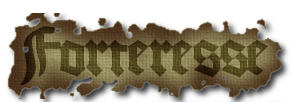
\includegraphics{coollogo_com-19602433.png}}
	\vfill{
	\centerline{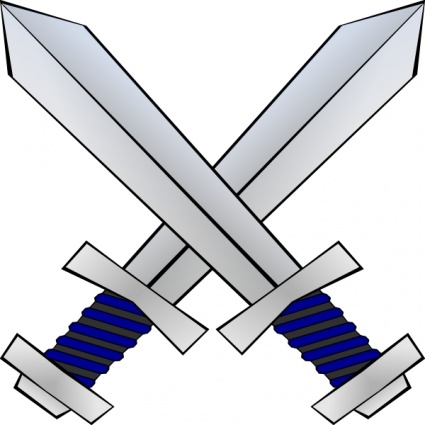
\includegraphics[scale=0.4]{crossed-swords-clip-art-48219.jpg}}}

    % Author and supervisor
    \begin{minipage}{0.4\textwidth}
      \begin{flushleft} \large	
      
      \end{flushleft}
    \end{minipage}
	\begin{flushleft}\vfill
      {
       \textsc{Chatelus} Florian - \emph{chatel\_f} \\
       \textsc{Henric} Arnaud - \emph{henric\_a}\\
       \textsc{Sarkar} Riday - \emph{sarkar\_r}\\
       }
    \end{flushleft}	
  \end{center}
  \end{sffamily}
\end{titlepage}


\shorttableofcontents{Sommaire}{1}
\newpage
\section{Introduction}
Dans le cadre de notre première année à EPITA, nous devons réaliser un projet informatique de fin d’année qui doit montrer l’application de nos connaissances dans le domaine de la programmation. Pour réaliser ce projet, nous avions formé un groupe composé de quatre étudiants. Actuellement, notre groupe n’est composé que de trois étudiants puisqu’un membre du groupe à quitté l’école.
Le sujet étant libre, nous avons décidé de réaliser un jeu vidéo nommé Forteresse. C’est un jeu du type \textit{Tower Defense}. La présentation du jeu est détaillée dans la reprise du cahier des charges.  
	\par Le présent document est  le rapport de projet  qui retrace les différents cheminements de création de ce projet  et il présente surtout le jeu.  Nous avons donc décrit les différentes tâches réalisées ainsi que les problèmes rencontrés et les solutions trouvées pour résoudre ces problèmes.
	\par Le plan de notre rapport sera divisé en trois parties. La première étant consacrée à la reprise du cahier des charges, la deuxième est consacrée à la présentation du jeu et la troisième, quant à elle, est consacrée au bilan personnel de chaque étudiant faisant partie de ce groupe.


\newpage
\section{Reprise du cahier des charges}
\subsection{Les origines du projet}
Nous avons choisi de réaliser un jeu plutôt qu’un logiciel car nous avons deux membres dans le groupe qui ont déjà réalisé un jeu en Terminale dans le cadre d’un projet en groupe. Même si le projet achevé en ISN par ces deux derniers n’est pas comparable avec ce qui nous attend ce semestre en INFO SUP, ce sera toujours une aide non-négligeable.
\par Une fois que la nature du projet était choisi, nous avons réfléchi longuement sur le type de jeu que nous allons réaliser. Notre expérience en tant que joueur nous donnait un large choix parmi les types de jeu possibles comme un RPG (Role Playing Game), RTS (Real Time Strategy) ou encore un Tower Defense . 

		\subsubsection{Présentation}
		\par Notre jeu sera basé sur le principe du \textit{tower defense}. Qu'est-ce que 			cela signifie? Un \textit{tower defense}, est un jeu qui comme son nom l'indique 			aura comme objectif de défendre un point donné. Le but du jeu sera donc de défendre 		un cristal qui alimente la porte de l'endroit que nous souhaitons protéger.  
		\subsubsection{Déroulement d'une partie}
		Une partie se déroulera en deux phases qui se répéteront, a chaque vague d'ennemis.\\
		\centerline{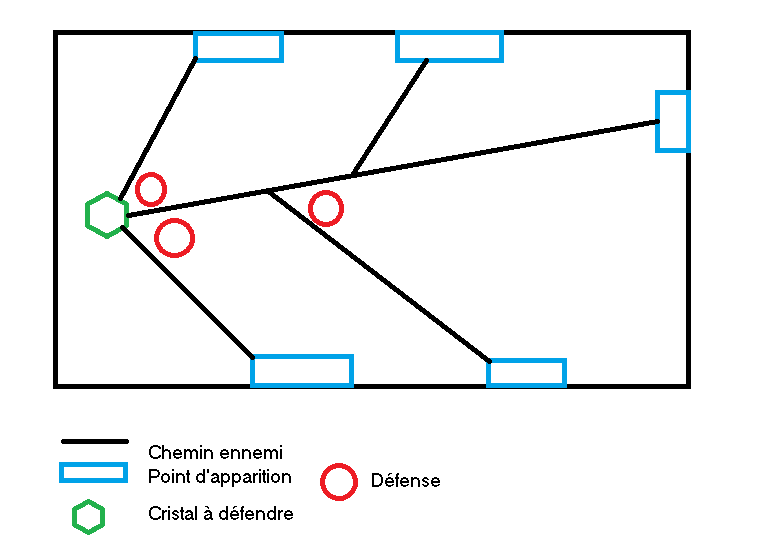
\includegraphics[scale=0.55]{Plan.png}}
		\par La première est la phase que nous appellerons \textit{phase de préparation}, elle consiste à préparer ses défenses, en les positionnant de façon stratégique, les améliorant ou en les réparant. Cette phase sera d'une importance capital pour assurer une victoire lors de la phase suivante. Une fois que vous serez fin prêt pour le combat, il vous suffira d'appuyer sur prêt et la deuxième phase commencera une fois tout les joueurs prêt.
		\par Nous arrivons donc en deuxième phase, la \textit{phase de combat}, qui va déclencher l'action. Des créatures vont apparaitre à des points précis de la carte et vont converger vers le ou les cristaux. Le joueur pourra donc durant cette phase attaquer les monstres et tenter de les détruire et/ou continuer à poser, améliorer et réparer ses constructions mais avec des malus d'incantation.
		\par Tous les certains nombre de cycle, au terme de ces deux phases, un monstre plus imposant apparaitra, et le joueur devra s'en défaire afin de remporter la manque et d'obtenir des objets.
		\subsubsection{Multijoueur}
		Le mode multijoueur consistera en un mode CO-OP. Vous devrez \^etre capable de jouer en \'equipe afin d'affronter vos adversaires. Pour cela, vous commencerez la partie c\^ote \'a c\^ote. Vous ne pouvez combattre seulement des IA. Le mode multijoueur consiste en un mode en \'equipe et non pas en 1vs1 contre un ami.
		\par Chaque joueur pourra int\'eragir avec l'environnement. Leurs constructions et leurs objectifs sont communs tandis que toutes leurs caract\'eristiques telles que leur monnaie et leur vie sont s\'epar\'ees.
		\subsubsection{L'interface}
		L’interface permettra au joueur d'être renseignée à tout moment sur : 
		\begin{itemize}
		\item Le temps écoulé.
		\item Sa jauge de vie.
		\item L’arme dont il est en possession , ainsi que les  munitions dont il dispose.
		\item L’argent qu’il possède pour acheter de nouvelles tours ou armes.
		\end{itemize}
		\subsubsection{L'arsenal de défense}
		Nous utiliserons donc différents types d’armes de type médiéval fantastique.
Les armes seront donc accessible en la ramassant sur un bosse ou bien  suite à un achat du joueur, elles pourront être améliorer, durant la partie. On distinguera plusieurs types d’armes tel que:
	\begin{itemize}
	\item Les épées.
	\item Les arcs.
	\item Les bâtons.
	\end{itemize}
Les défenses fixes seront achetable grâce a l’argent gagné durant la partie. Les défenses seront comme les armes améliorables. Ces dernières seront autonomes et feront partie de l’IA. On pourra y trouver:
	\begin{itemize}
	\item Des tourelles.
	\item Des pièges.
	\item Des auras.
	\end{itemize}
\newpage
\subsection{Découpage du projet}
	\subsubsection{Le graphisme}
		\subsubsection{La 3D}
		Étant donné sa gratuité, nous allons utiliser Blender pour réaliser des modèles 3D. Ce logiciel va nous permettre de modéliser les différents personnages de notre jeu et de faire les diverses textures de l’environnement du jeu.

		\subsubsection{La 2D}
		La 2D de notre jeu sera principalement représenté par l'interface graphique du joueur. En effet, le joueur aura besoin d'avoir des informations et de repère visuel afin d'interagir correctement avec son environnement et d'avoir une expérience de jeu la meilleure possible. La 2D pourra également jouer un rôle important dans les menus
	\subsubsection{Audio}
	L’audio gère évidemment tous les sons. De bruitages dans le jeu à musique dans les menus, nous devrons trouver des sons qui s’adaptent au contexte médiéval.

	\subsubsection{Le réseau}
	Le réseau consistera tout simplement a implémenter un mode multijoueur, afin que les joueurs puisse jouer ensemble en ligne ou bien en réseau local.
	\subsubsection{L'intelligence artificiel}
	Pour définir l’IA, nous allons créer différents niveaux de difficultés. Le but est que l’IA détruise le cristal que nous devons protéger, ainsi, l’IA est l’ennemie. Il contrôle plusieurs personnages. Nous devons coder un IA capable de se déplacer vers le cristal, mais également de combattre contre l’utilisateur, de mourir tué par le héros ou les tourelles. 

	\subsubsection{Le menu}
	Nous tenterons de créer un menu accessible et design. Il devra permettre d'accéder au lancement d’une nouvelle partie, aux options, ainsi qu’au mode multi-joueur. 
	\subsubsection{Le site}
	Modéliser un site web avec une présentation générale des créateurs et de la création (chronologie, problèmes, solutions…). Ajouter des images du jeu. Expliquer les règles.  Donner les références utiles pour notre réalisation. Permettre le téléchargement du jeu aux utilisateurs, et mettre à disposition le rapport ainsi que le jeu en version lite.
	\subsubsection{Gameplay}
	Le gameplay consiste à coder tous les mouvements de notre héros, soit le personnage que l’on contrôle… Il devra être capable de donner des coups, construire des tours, courir, sauter, et bien sûr, se déplacer à n’importe qu’elle point accessible de la map. Le gameplay consiste également à coder la caméra suivant notre héros. Ce jeu se jouant à la troisième personne, la caméra devra être capable de toujours regarder le héros de derrière et de le suivre dans tous ses mouvements. On devra ici géré également tous les problèmes de collision.
	\subsubsection{Animation}
	L’animation est le moyen de rendre les mouvements des personnages fluides et réalistes. Chaque mouvement devra être animé, les jambes lorsqu’un personnage se déplace, les bras lorsqu’il combat, etc...

\newpage

\subsection{Répartition des tâches}
Nous avons décidé d’attribuer chaque tâche à au moins deux personnes car ainsi chaque membre réalise plusieurs tâches et peut apprendre des choses de domaines différents . De plus, si un membre rencontre des difficultés et se retrouve bloqué pour réaliser une tâche, son coéquipier peut venir en aide puisqu’ils s’occupent de la même tâche. Ainsi la réalisation des tâches devient plus facile.
\bigbreak
\bigbreak
\begin{center}
	\begin{tabular}{|c||c|c|c|c|c|}
		\hline
		& Florian & Riday & Arnaud \\
		\hline
		Site &  & $\times$ & $\times$\\
		\hline
		3D &  $\times$ & $\times$ &\\
		\hline
		2D & & $\times$ & $\times$\\
		\hline
		IA & $\times$ &  & $\times$\\
		\hline
		Multijoueur & $\times$  & $\times$ &\\
		\hline
		Réseau & $\times$ & $\times$ &  \\
		\hline
		Menu & $\times$ & & $\times$\\
		\hline
		Gameplay & $\times$ & $\times$ &\\
		\hline
		Animation & $\times$ & & $\times$\\		
		\hline
		Audio & & $\times$ & $\times$\\
		\hline
		\LaTeX & $\times$ & $\times$ & $\times$ \\
		\hline
	\end{tabular}
\end{center}
	\newpage
\subsection{Ressources utilisées}
	\subsubsection{Ordinateur}
	Nous utiliserons a l'évidence des ordinateurs. Ils seront notre principale outil de travail. Nous utiliserons un ordinateur dans toutes les étapes de notre projet. 
	\subsubsection{Visual Studio 2015}
	Visual Studio est le logiciel qui nous permettra de coder nos script sur Unity. Nous l'utiliserons plus particulièrement afin d'utiliser le langage C\# qui représentera la quasi-totalité, voir la totalité de notre code.
	\subsubsection{Unity}
	Unity sera LE logiciel cœur de notre projet, il lui servira de base. Il nous permettra de mettre en relation des objets avec des scripts que ces objets effectuerons. Ce logiciel correspond parfaitement a nos besoins, dans la réalisation d'un jeu vidéo. De plus il possède une courbe d'apprentissage linaire et est facile d'accès, ce qui correspond a nouveau avec notre statut d'étudiant en première année.
	\subsubsection{Gimp/Blender}
	Gimp est un éditeur graphique. Il nous sera utile notamment pour la création de la 2D, et donc de l'interface graphique de notre jeu. Sans oublier la jaquette de notre jeu lorsqu'il sera en version CD.
	\par Blender quant a lui est un logiciel de modélisation 3D et sera simplement destiné a la création d'éléments 3D pour notre jeu. 
	\subsubsection{Tutoriel}
	Enfin, la ressource que nous utiliserons le plus, après nos ordinateurs, sont les tutoriels. Dans la mesure où, cette expérience est inédite pour chacun d'entre nous, nous aurons besoin d'acquérir de nombreuse connaissance. C'est ici qu'interviendront les nombreux tutoriels à notre disposition sur le web. Notez que des tutoriels on été visionné pour la réalisation de ce cahier des charges.
\subsection{Planning}
	\begin{tabular}{|c||c|c|c|}
		\hline
		& 1\iere{} soutenance & 2\ieme{} soutenance & 3\ieme{} soutenance \\
		\hline
		Site &  Avancé & Avancé & Terminé \\
		\hline
		3D & Débuté & Avancé & Terminé \\
		\hline
		2D & Débuté & Avancé & Terminé \\
		\hline
		IA & Débuté & Débuté & Terminé\\
		\hline
		Multijoueur & Débuté & Avancé & Terminé\\
		\hline
		Réseau & Débuté & Avancé & Terminé\\
		\hline
		Menu & Avancé & Terminé & Terminé \\
		\hline
		Gameplay & Débuté & Débuté & Terminé\\
		\hline
		Animation & Débuté & Avancé & Terminé\\		
		\hline
		Audio & Non débuté & Débuté & Terminé\\
		\hline		
	\end{tabular}\\
	\newpage
\subsection{Budget}

Nous sommes des étudiants et ceci est un projet de première année. C'est donc un projet dans le cadre scolaire et à but non lucratif. Ainsi, le budget sera de 0\euro{}. Aucun achats ne sera nécessaire à la réalisation de notre projet. Les dépenses seront donc également de 0\euro{}. Seul des logiciels gratuits ou bien fournit gratuitement par l'école seront utilisés dans ce projet. Un léger dépassement de budget est bien entendu possible, notamment pour l'achat d'un CD si cela s'avère nécessaire.\\
\centerline{
\includegraphics[scale=0.7]{images.jpg}}
\newpage
\section{Le jeu}
	\subsection{\textsc{Sarkar} Riday}
	
	\subsubsection{Graphisme}
Le graphisme occupe une place de plus en plus importante dans les jeux-vidéos. En effet, la plupart des jeux provenant de ténors du marché vidéoludique se veulent de plus en plus réaliste. Nous avons donc essayé d’avoir des graphismes réalistes.

\paragraph{La 2D}
Au début du projet, j’avais des difficultés avec cette partie mais des lorsque l'on a compris le fonctionnement de la 2D sur Unity, on ne rencontre aucune difficulté à faire cette partie. Pour cette partie, j’ai dû attendre que Florian soit assez avancé dans les parties Gameplay et l’IA. Par exemple, j’avais mis en place les barres de vie et l’affichage du gain du joueur mais j’ai dû attendre un peu pour les rendre fonctionnels. J’ai dû aussi comprendre avec des explications, les codes de Florian pour réaliser ma partie de 2D.
\par Avec l’accord de Florian, pour l’interface du jeu, j’ai essayé d’aider au mieux le joueur. Pour cela, je me suis renseigné auprès des personnes qui jouent régulièrement aux jeux-vidéos et j’ai appris que lorsqu’on commence un nouveau jeu, il arrive qu’on oublie certaines touches. Pour aider le joueur, j’ai donc décidé de rappeler les touches principales par le biais d'un système d’affichage. Pour que le joueur puisse comprendre le contexte du jeu et ses missions, j’ai aussi rappeler par un affichage ce qu’il doit faire pour commencer la partie. Par exemple, lorsqu’on commence une partie, le jouer sait par les affichages qu’il s’agit de défendre le cristal et pour le défendre, il doit commencer par placer des tours puis lancer une vague. Le joueur sait aussi les différents moyens de défenses dont il peut se servir ainsi que leur prix et les touches sur lesquelles il faut appuyer pour utiliser les différents moyens de défenses. En jouant \`a notre jeu, nous nous sommes rendu compte qu’il n’y a aucune indication pour le début et la fin d’une vague. J’ai ajouté donc des affichages qui indiquent le début et la fin d’une vague. Le joueur peut aussi voir le numéro de la vague en cours.
\par Nous avons deux barres de vie : une destinée pour la vie du joueur et l’autre pour la vie du cristal. Pour distinguer les deux barres de vie, j’ai décidé de placer un guerrier devant la barre de vie du joueur et un cristal devant la vie du cristal. Pour la partie 2D, j’ai utilisé essentiellement deux logiciels du traitement d’images qui sont Paint et GIMP.\\
\begin{figure}[!ht]
\centerline{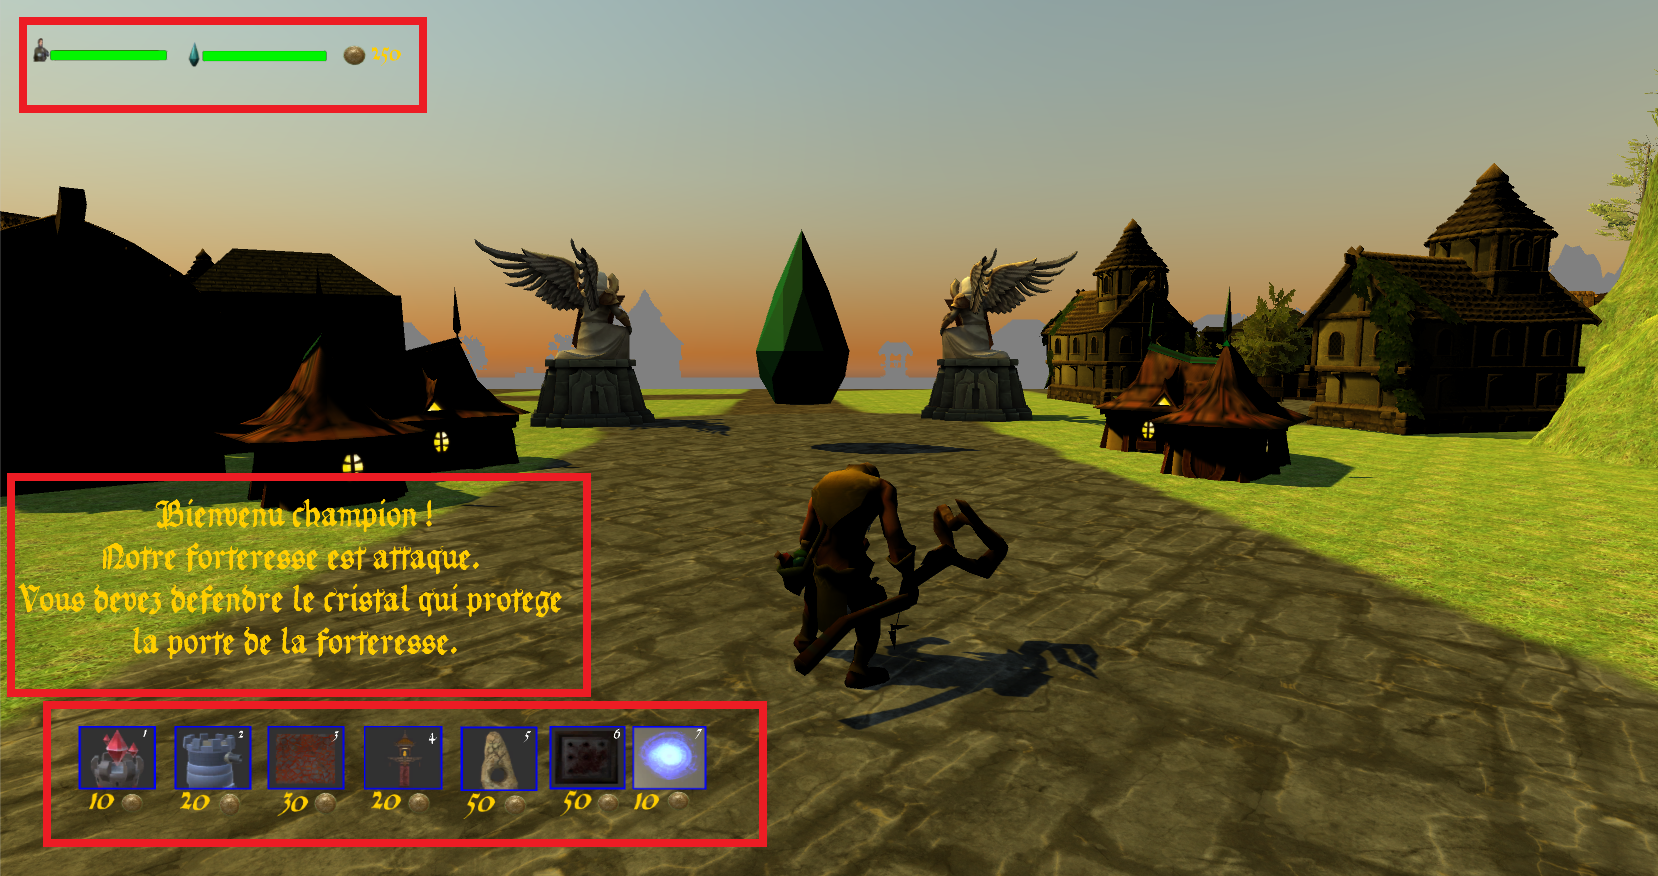
\includegraphics[scale=0.3]{interface2D.png}}
\caption*{Interface 2D}
\end{figure}
\subsubsection{La 3D}
Au début du projet, je me suis occupé tout seul de cette partie mais au cours de la réalisation du projet, Florian m’a rejoint. Au début du projet, je voulais modéliser les personnages mais comme on a décidé un jeu avec un graphisme plutôt réaliste, on a décidé de prendre les modèles de personnages de l’asset  store mais puisque le cristal est un élément majeur de notre jeu, je l’ai modéliser en passant par le logiciel de modélisation 3D Blender. Puis avec Unity, j’ai ajouté une texture. Après la deuxième soutenance, monsieur Van der Laere nous a conseillé de multiplier les personnages et les différents moyens de défenses. Nous avons deux modèles de personnages et plusieurs modèles d’ennemis. Nous avons trouvé qu’il n’est pas intéressant de les faire apparaitre tous les modèles d’ennemis dans la même vague donc pour voir tous les modèles, il faut finir plusieurs vagues.
\par Pour lancer le projet, j’ai modélis\'e les deux cartes puis j’ai ajouté des détails sur les deux cartes avec Florian. Pour la première carte, nous avons un terrain plutôt vert entouré de chaines de montagnes car entourer le terrain par des chaines de montagnes rendait le terrain plus joli. Puis avec des textures de roches j’ai dessiné des chemins qui vont être empruntés par les ennemis. Nous avons plusieurs points d’apparition d’ennemis et donc ils suivent des chemins différents pour venir attaquer le cristal. Pour la deuxième carte, Florian était du même avis que moi pour r\'ealiser un terrain plutôt urbain. J’ai donc décidé de changer les textures. J’ai ajouté des textures de briques pour rendre le terrain urbain. J’ai chang\'e aussi les textures de roches pour les chemins dans la deuxième carte.
\begin{figure}[!ht]
\centerline{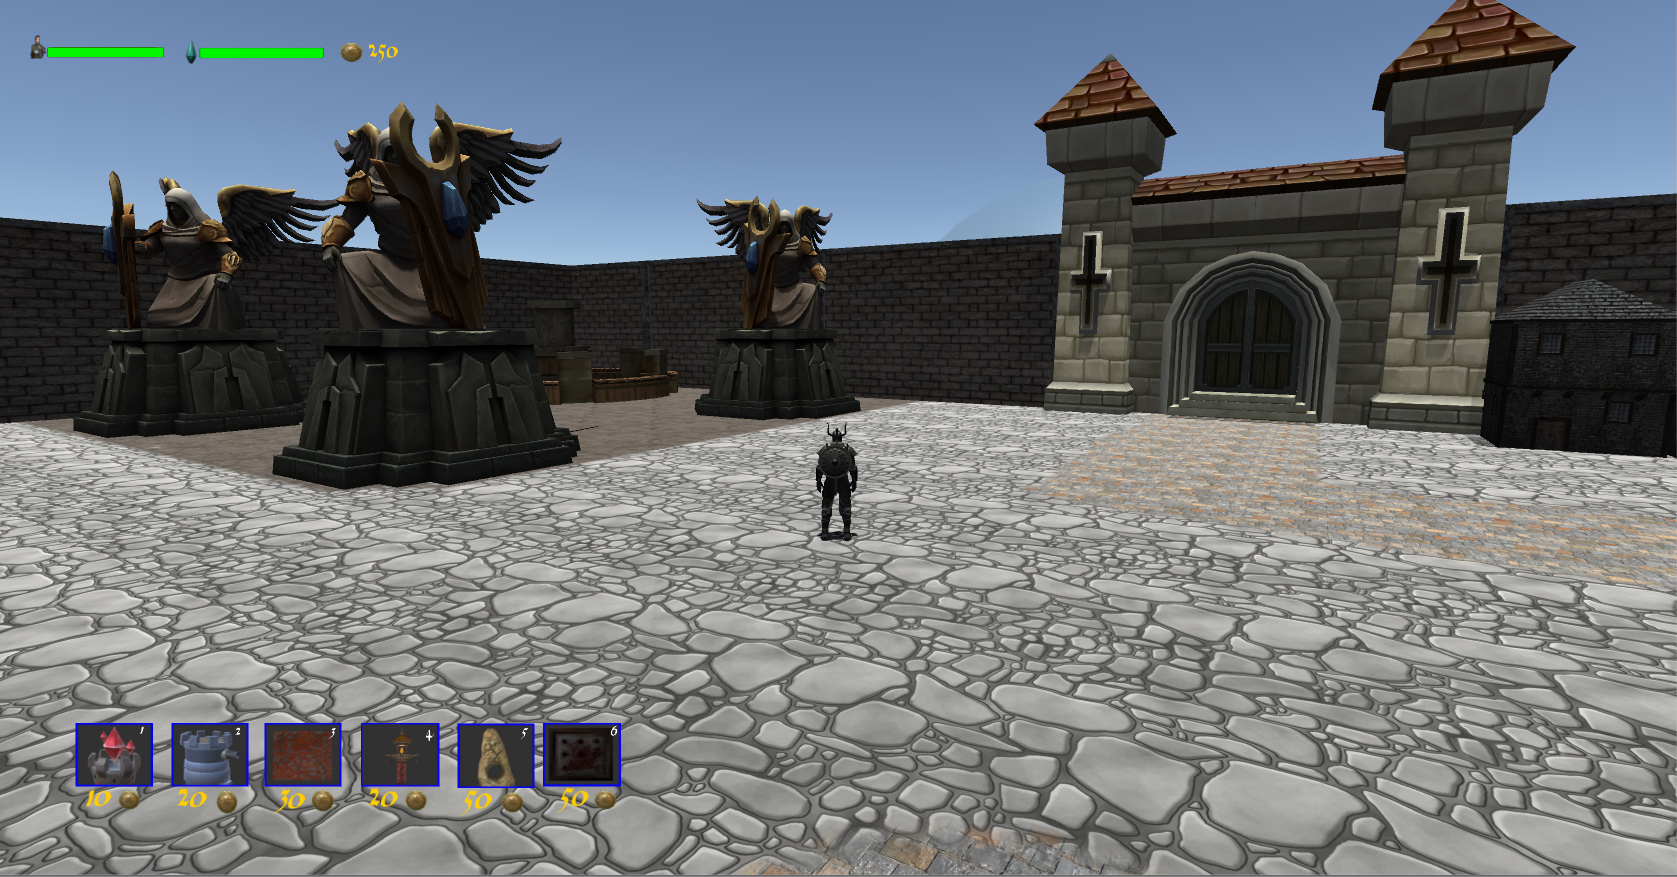
\includegraphics[scale=0.3]{3Dmap2.png}}
\caption*{Base de la deuxi\`eme carte}
\end{figure}
	\subsubsection{Reseau}
\par Obtenir un mode multijoueur a été l’objectif que je m’étais fixé pour la soutenance finale parce que j’ai eu beaucoup de difficultés. Pour cette partie, j’ai regardé beaucoup de tutoriels qui utilisent des méthodes différentes. J’ai mis en place un réseau en mode host en utilisant l’Unet d'Unity. Un joueur se porte comme serveur et les autres joueurs peuvent le rejoindre en tant que clients. On a fixé 4 clients par serveur. Pour cette partie, j’ai dû modifier tous les scripts avec la participation de Florian afin de gérer le mode multijoueur. Ainsi notre jeu a maintenant la possibilité de gérer plusieurs joueurs en même temps sur une carte.
\par La principale difficulté a été pour moi l’adaptation des scripts pour le mode multijoueur, mais aussi des éléments de notre jeu. En effet, les joueurs ainsi que les différents éléments de notre jeu doivent être synchronisés. Il est compliqué de choisir les informations à envoyer au serveur (vie, positions, déplacement, etc...).

\subsubsection{Le Multijoueur}

Pour la partie multijoueur, j’ai mis en place un système de chat qui permet la communication entre les différents joueurs. Comme il est très important de placer les tours dans des endroits stratégiques, nous pensons que ce système de chat est très utile pour les joueurs.
\begin{figure}[!ht]
\centerline{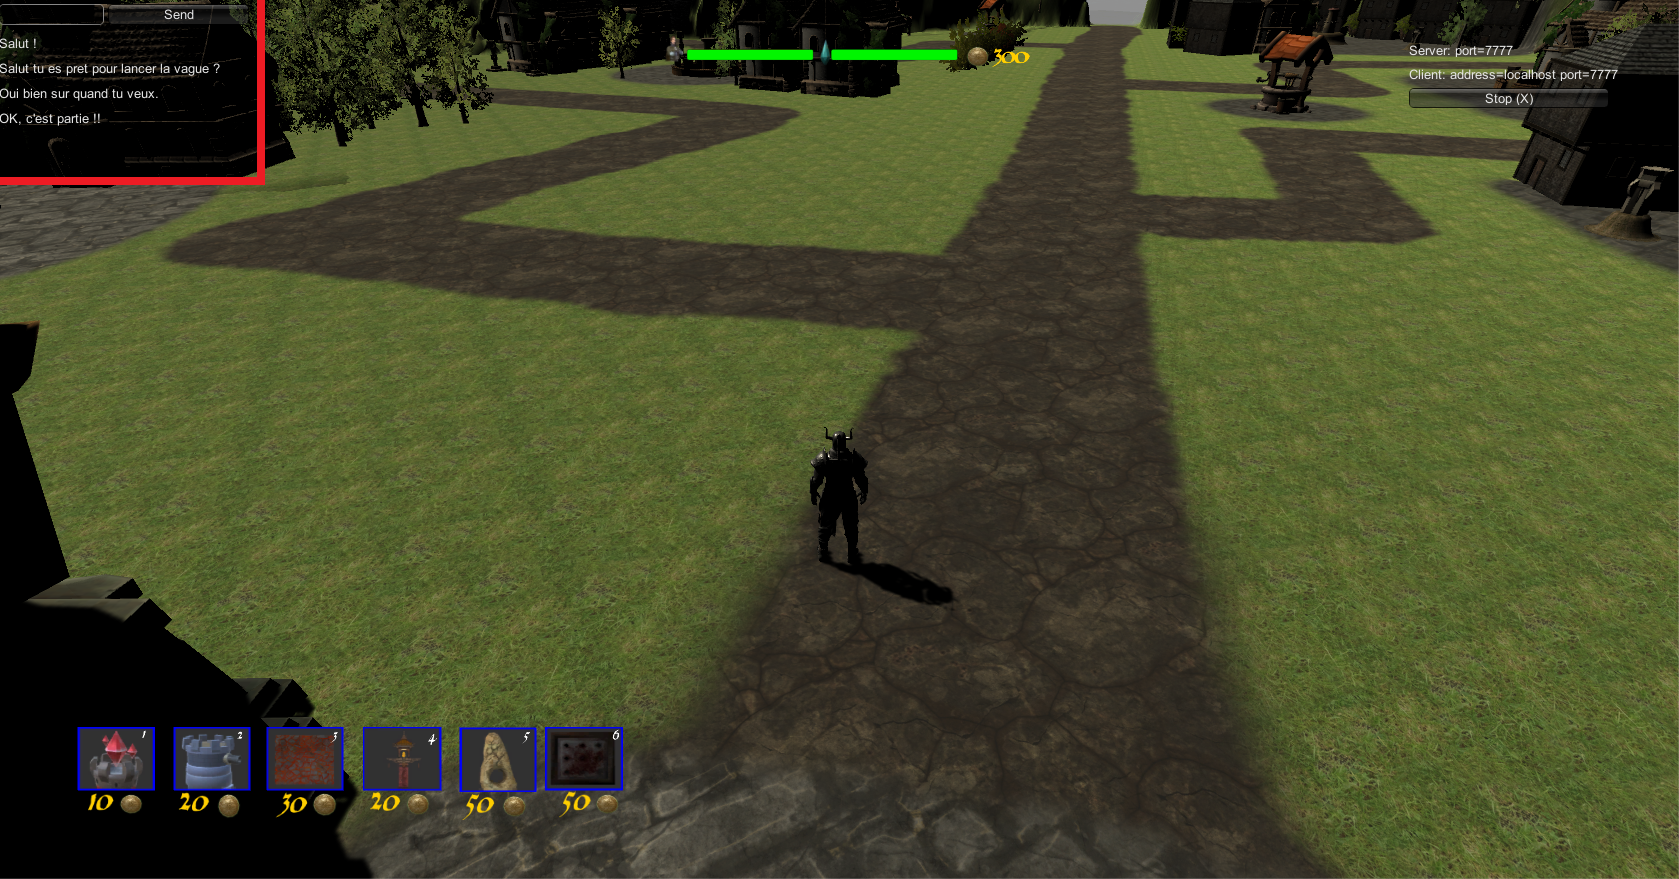
\includegraphics[scale=0.3]{Chat.png}}
\caption*{Un joueur communicant avec un autre joueur gr\^ace au chat}
\end{figure}
\subsubsection{Le site internet}
Pour cette partie, j'ai fait un historique qui r\'ecapitule les r\'ealisations majeures de notre projet pour les mettre sur le site.


	\subsection{\textsc{Henric} Arnaud}
	\subsubsection{Histoire et bande annonce}
	Forteresse n’est pas seulement un \textit{tower defense} consistant à éliminer des ennemis et protéger un cristal. Nous avons essayé de proposer un scénario crédible et attirant pour les joueurs potentiels. En effet, le mage, le héros et les cartes ont une histoire et notre but était de ne rien laisser au hasard. On voulait créer des liens entre les héros et le monde qu’ils défendent mais également avec l’ennemi. Le but, qui est de défendre un cristal dans une partie, devait être explicable. L’important est que le joueur, au moment de lancer le jeu, soit au courant de toute l’histoire et ressente en quelques sortes, l’urgence de repousser ces ennemis. C’est pourquoi nous avons décidé de réaliser une vidéo d’introduction que nous pourrons visionner avant le lancement d’une partie pour susciter l’attention du joueur et le mettre dans l’ambiance de Forteresse.

		\subsubsection{Site internet}

Nous pensons que le site internet est une partie presque aussi importante que le jeu en lui-même. Effectivement, il représente le premier contact avec nos futurs joueurs. On devait donc réaliser un site avec un design en accord avec notre jeu et qui nous motive à le télécharger. Nous devons aussi réaliser un site fonctionnel, organisé et facilement accessible évidemment. Pour ma part, j’ai donc créé une page d’accueil dynamique et expliquant en bref Forteresse comme pour une publicité. Ensuite, en cliquant sur les différents liens, on peut avoir accès à différents onglets. Parmi ces différents onglets, on distingue une page de présentation du jeu et de ses règles, accompagnés par des images tirées du jeu directement. Ensuite, on peut accéder à une page où l’on informe de tous les outils utilisés pour la réalisation du projet associés avec un lien renvoyant tous vers leur site officiel. On a évidemment une page de téléchargement du jeu. Les liens renvoient vers le fichier d’installation du jeu en version complète ou condensé ainsi qu’un lien pour télécharger le cahier des charges. Enfin, un autre onglet concerne l’avancée dans la réalisation du projet au fil des semaines depuis le premier jour.

		\subsubsection{Les Menus}

Le menu prend une place importante dans le jeu puisqu’il apparait en premier lors du lancement et permet de tout lier. Il doit être fonctionnel et facilement accessible. Le menu principal peut donc lancer le jeu en mode un joueur ou multijoueur mais il possède également un menu d’options et permet aussi de quitter Forteresse. J’ai souhaité rendre ce menu beau et dynamique, c’est pourquoi j’ai mis en fond les cartes de notre jeu. Ensuite, lors du lancement d’une partie, on accède d’abord à deux menus : un menu de sélection de la carte puis un second menu pour sélectionner le personnage que nous souhaiterons contrôler. Ainsi, on peut jouer sur la carte que l’on souhaite et choisir le héros ou le mage. Enfin dans une partie, en appuyant sur “échap”, nous avons le menu pause qui s’affiche. La partie est donc naturellement en pause et les personnages s’arrêtent. Dans ce menu, on peut quitter la partie, la relancer, quitter le jeu ou bien-s\^ur, reprendre la partie en cours en appuyant sur les boutons correspondants. Enfin, j’ai également créé un menu de victoire et de d\'efaite qui s’affichent respectivement lorsque le cristal a encore de la vie à la fin de la dernière manche ou lorsqu’il est détruit. Si le héros meurt, nous indiquons également au joueur qu’il doit attendre quelques secondes avant de revivre.
\begin{figure}[!ht]
\centerline{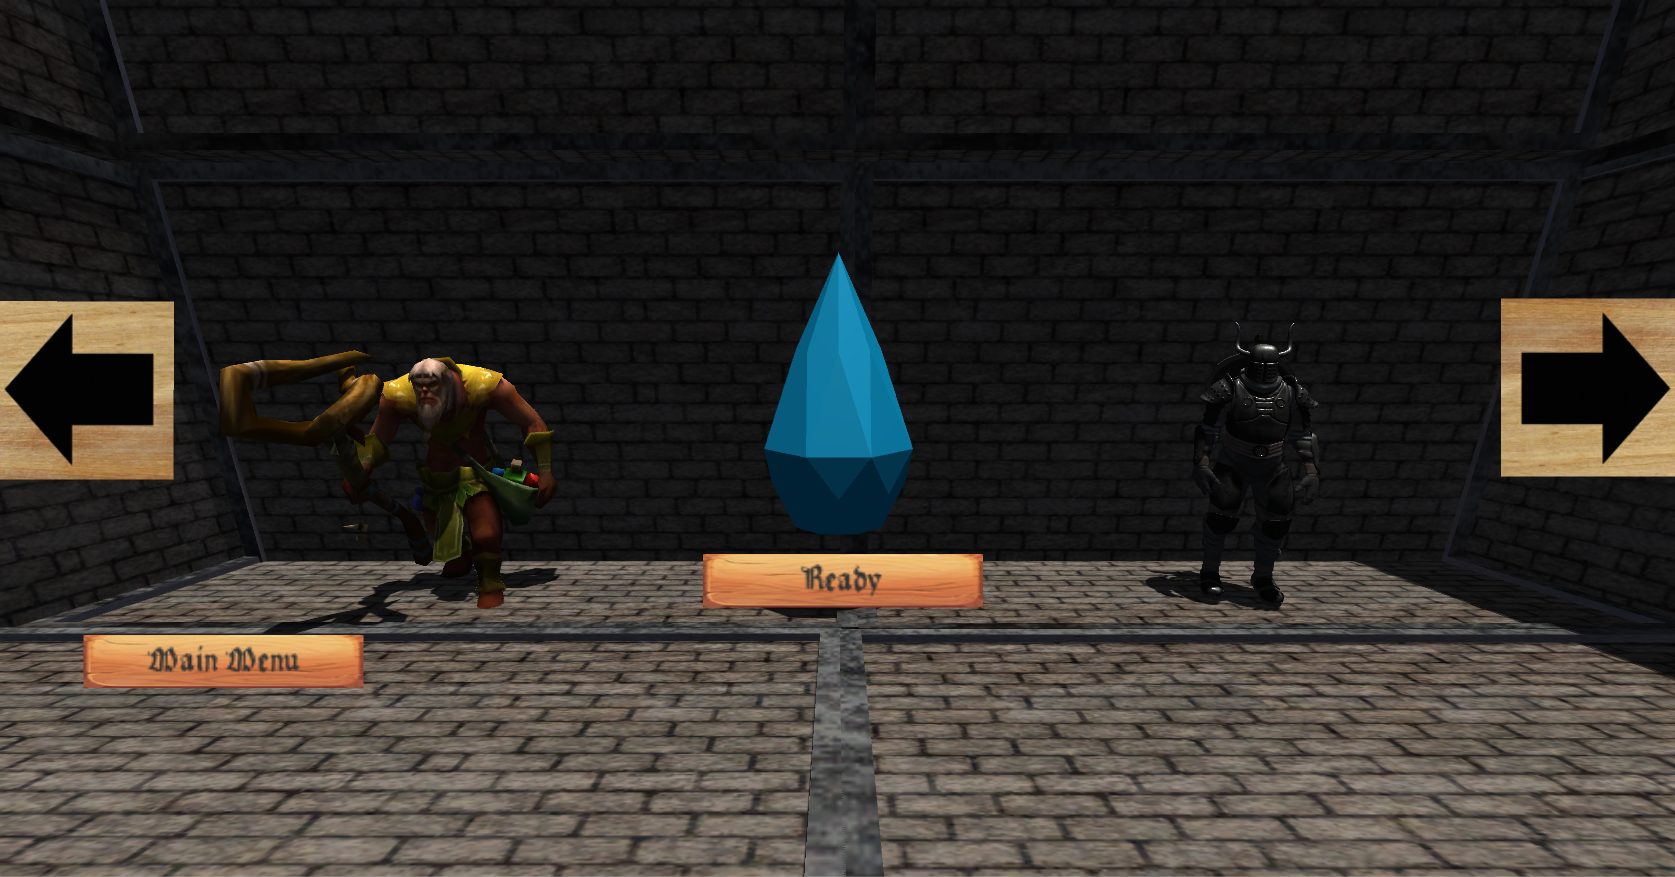
\includegraphics[scale=0.3]{selectionDesPersonnages.png}}
\caption*{Menu s\'election des personnages}
\end{figure}

		\subsubsection{L'intelligence artificielle}

La partie intelligence artificiel concernait pour ma part la gestion des animations en fonction des agissements des ennemies. En effet, les monstres devaient marcher lorsqu’ils se déplacent, donner des coups lorsqu’ils attaquent, tirer des flèches lorsque l’archer est dans une zone de combat ou encore, mourir lorsque l’ennemi n’a plus de vie. Pour cela, je devais assurer la bonne gestion entre les animations et mouvements de chaque personnage pour rendre Forteresse encore plus réaliste.

		\subsubsection{Les Animations}

Les animations représentent la partie la plus cruciale pour rendre un jeu réaliste. Un jeu peut être fonctionnel mais s’il n’est pas dynamique, il n’attire pas les joueurs longtemps. C’est pourquoi, on devait bien faire en sorte de lier les mouvements des personnages avec les évènements sur le terrain et des touches sur lesquelles nous appuyons. Dans un premier temps, on devait animer le héros que l’on déplace. Ses animations dépendent effectivement du mouvement effectué : s’il se dirige vers l’avant, à gauche, à droite, en arrière mais également, s’il effectue des mouvements en diagonales. Bien sur, lorsqu’il attaque un ennemi, on le voit donner des coups si on clique sur le bouton correspondant. Enfin, le héros peut également sauter et mourir avec des animations appropriées.
\par Dans un second temps, tous les différents ennemis sont également animés lorsqu’ils marchent, attaquent ou meurent. A noter que les animations varient pour tous les différents types d’ennemis. En effet, l’archer envoient des flèches alors que le squelette donnent des coups d’épées et les gobelins, des coups de poing. La diversité des animations nous semblait importante pour ajouter davantage de réalisme.

		\subsubsection{L'Audio}

La partie audio, sans être forcément évidente à réaliser, n’était pas la partie prioritaire même si comme pour les animations, elle contribue au réalisme du jeu. Dans le menu, nous pouvons écouter en fond la musique du jeu, on peut également régler le volume dans les options.
Pour tous les différents mouvements, on devait ajouter un effet sonore différent. 
\par L’audio permet également de nous rapprocher avec le contexte médiéval et épique repris dans le scénario avec des bruitages de coups d’épée ou de magie que nous entendons pas dans notre époque.

	\subsection{\textsc{Chatelus} Florian}
		\subsubsection{Le scenario}
		Un bon jeu se doit d’avoir un scenario, permettant de justifier les aventures du héros et de permettre aux joueurs de mieux s’identifier aux personnages. Il est vrai qu’avoir un scénario n’a pas été notre priorité numéro un, mais cela nous a tout de même paru important. De plus, notre jeu est ancré dans un univers fantastique, qui a permis de laisser voguer nos imaginations. Avec Arnaud nous avons créé cet univers, et élaboré un scenario afin qu’il puisse être le plus cohérent possible. Le scenario est inspiré des nombreux univers fantastiques que j’ai pu rencontrer, avec notamment \textit{Le seigneur des anneaux}, \textit{Warcraft} ou même \textit{Harry Potter}. L’un des objectifs de la création d’un scenario était de permettre de se projeter dans l’univers afin d’imaginer des suites possibles à notre jeu.
\par Au début du jeu, vous pouvez incarner deux personnages, un mage qui est le personnage principale de notre intrigue et un guerrier qui est un de ses amis qui s’apprête à rejoindre l’armée royale. C’est au moment des adieux que le village est mystérieusement  attaqué par des créatures encore jamais vue auparavant, du moins c’est ce que l’on pourrait croire. C’est ainsi que commence l’histoire de nos deux héros.
\par Pour le moment, l’univers de notre jeu est limité mais dans les possibles suites du jeu, le joueur sera amené à découvrir de plus en plus l’histoire du monde dans lequel il évolue. En effet, les deux premières cartes, que nous avons créées, ne se situent qu’au début de l’intrigue, ce n’est que le village natale des deux héros. Ils seront amenés à parcourir le monde entier afin de vaincre le mal inconnu qui frappe leurs villages et le reste du monde.
		\subsubsection{Le Graphisme 3D}
		
		Forteresse est un jeu en 3D et comme dans tous jeux, il y a une interface graphique. Nous avons choisis de créer deux cartes, cela était suffisant au vu de nos capacités. Créer plus de cartes aurait été d’un intérêt moindre et aurait été néfaste pour le jeu, puisqu’il nous aurait empêché de consacrer du temps à la création de nouveaux monstres ou de nouveaux outils de défense. 
\par Je me suis personnellement occupé de la réalisation des cartes en y habillant le terrain de bâtiments et de décorations. Pour la réalisation de ces cartes nous avons veillé à respecter une certaine homogénéité  et continuité avec le scenario. 
\par Etant donné que la taille de notre groupe a été réduite, suite à un départ, nous n’avons pas eu les ressources humaines nous permettant de réaliser nos propres modèles. Nous avons donc dû effectuer une sélection parmi les modèles à notre disposition, afin qu’ils soient un maximum cohérent entre eux et avec notre univers. Ceci compose la majeure partie de la 3D dont je me suis occupée avec l'agencement des objets sur la carte.
La première carte est située devant le village natal des héros, on peut y voir une porte, c’est une des nombreuses portes qui mènent à son village. On peut voir un cristal devant la porte – c’est l’élément principale du jeu – qui alimente en énergie la porte et qui la protège. Sur le reste de la carte, on peut observer des habitations en dehors du village qui lui, est protégé par des remparts.
\par La seconde carte, est le village en lui-même. Il est protégé par des remparts et possède deux cristaux qui protègent les habitations à l’intérieur de l’enceinte des murs. Il est plus urbain, c’est presque une ville. Le village possède des remparts, pour le protéger puisqu’il se situe aux abords de nombreuse forêts. Des monstres dangereux peuvent y résider comme les gobelins ou les trolls. Des puits, sont présent afin d’assurer les besoins en eau de la population. On peut également y voir des cimetières, ceux-ci sont présents à l’intérieur de l’enceinte du village, pour éviter les pillages gobelins. 
\par Dans les deux cartes, on peut observer la présence de statues d’ange ; elles sont là pour permettre aux héros de réapparaitre en cas de mort.

\begin{figure}[!ht]
\centerline{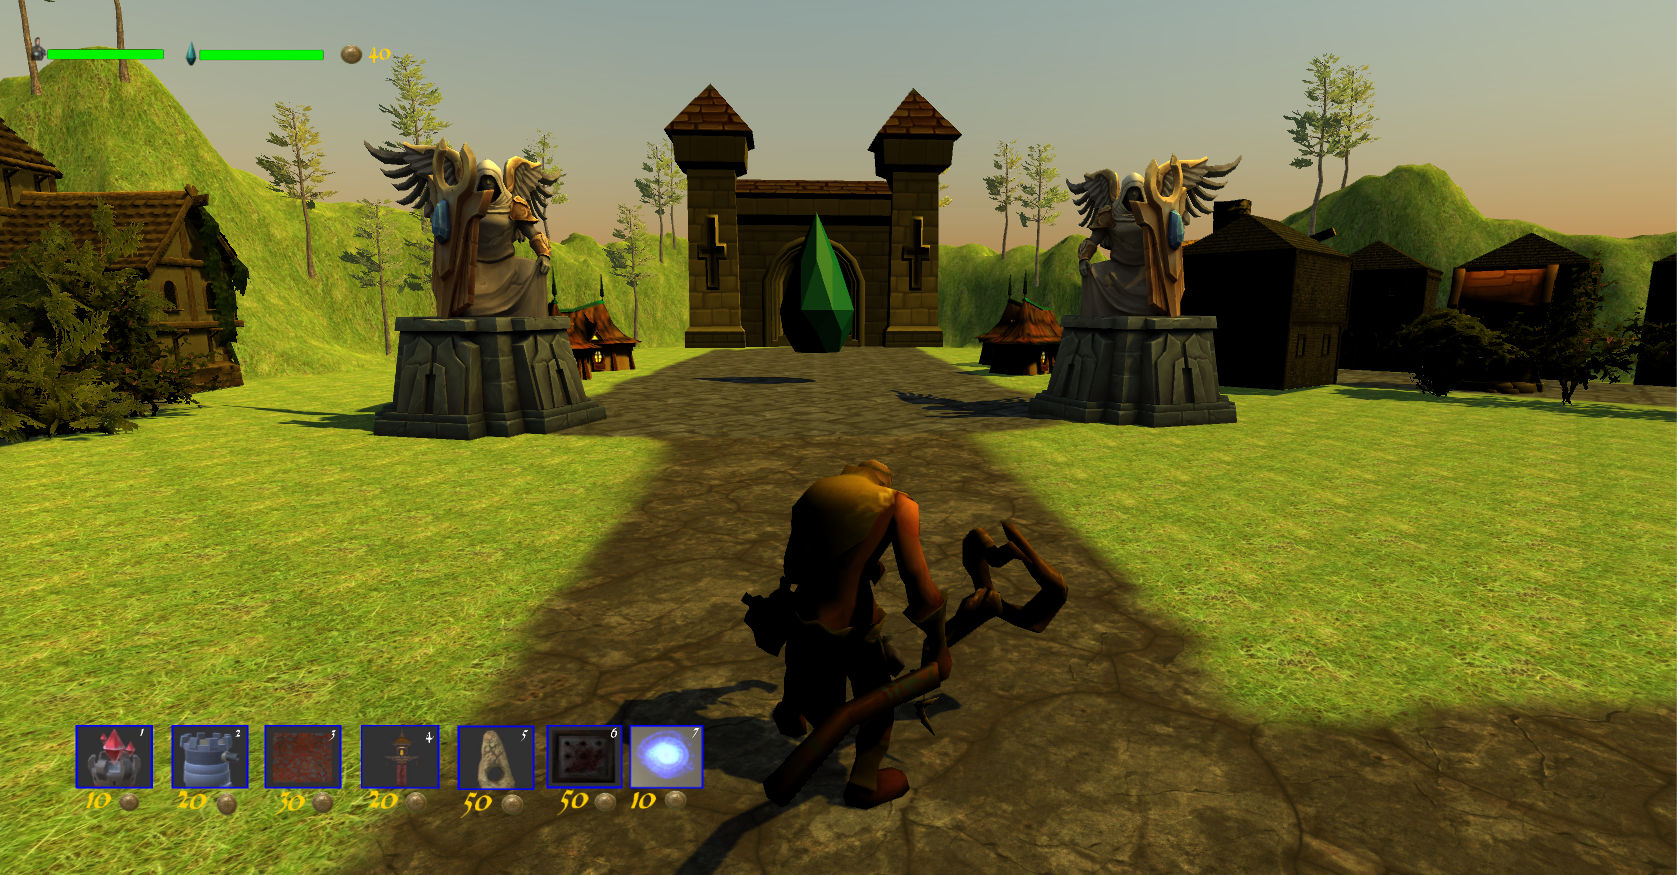
\includegraphics[scale=0.3]{3D.png}}
\caption*{Base de la premi\`ere carte}
\end{figure}
		\subsubsection{L'intelligence artificielle}
		L’intelligence artificielle ou IA est ce qui va permettre aux personnages non-joueurs d’effectuer des actions, comme se déplacer ou attaquer. 
\par Tout d’abord, les ennemis de notre jeu ont besoin, contrairement à nos tours de se déplacer. La première étape est donc de permettre à nos ennemis de se déplacer mais pas de n’importe quelle façon, les ennemis doivent suivre la route qui leur est destinée. Il faut donc que l’ennemi sache quelles routes il doit suivre, chose qu’il détermine en fonction de sa position et de son point d'apparition. Suivre un chemin c’est bien, mais nous voulions que nos ennemis soit capable de faire plus, nous voulions qu’ils puissent être attiré par le joueur et qu’ils puissent le poursuivre. Il a fallu permettre à l’ennemi de savoir quand un joueur passait trop proche de lui et qu’il devait se mettre à le suivre. Cependant, une fois qu’il est capable de suivre ce joueur, il a fallu lui indiquer à quel moment il devait décider que l’ennemis était trop loin et qu’il devait abandonner la poursuite. On pourrait croire que l’ennemi va désormais suivre correctement le joueur, mais il faut également lui indiquer à quelle distance du joueur, l’ennemi doit s’arrêter pour ne pas lui rentrer dedans. Ce dernier point prend tout son sens notamment dans le cas des archers, en effet nous ne voulons pas que des archers se retrouve au corps à corps, il faut donc leur dire à quelle distance ils doivent s’arrêter pour tirer.
\par L’étape finale pour nos ennemis a été de leur permettre de remplir leur fonction première, c’est-à-dire d’attaquer ! Il faut alors à nouveau dire à l’ennemi s’il est assez proche pour lancer son attaque ou non.

		\subsubsection{Le Gameplay}
			\paragraph{Les personnages}
			Comme décrit dans le scénario, notre jeu possède deux héros. Nos deux personnages sont capables de se déplacer, sauter, d’attaquer et d’utiliser l’arsenal de défense. Cependant, il existe des caractéristiques qui diffèrent selon le héros.
\par Le mage est un héros qui porte des habits en toile, il est donc plus vulnérable, il possède un montant de point de vie relativement faible en comparaison avec le guerrier. Bien qu’il soit peu résistant il dispose néanmoins de puissants atouts, notamment en attaque. 
Il possède la capacité d’envoyer des boules de feu à l’aide de son bâton, afin de lui permettre de combattre les ennemis à distance. Les boules de feu envoyé par le mage, se dirigent en ligne droite dans la direction visée.
\par Le guerrier possède une armure en plaque, robuste et à toute épreuve. Cela lui confère un nombre important de points de vie. Sa robustesse lui permet d’aller se battre au corps à corps. Il peut alors user de ses poings afin de défaire les ennemis, même les plus robustes. Son attaque au corps à corps possède une zone de dégâts bien plus important que celle du mage, il sera donc extrêmes puissant lorsque de multiples ennemis de faible puissance lui feront face.
			\paragraph{Les ennemis}
			Notre jeu possède de nombreux ennemis, qui possèdent tous des caractéristiques différentes.\\
			
\par Les squelettes, sont des créatures invoquées pas les démons, ou les nécromanciens. Ce sont des unités de base qui servent principalement de chair à canon. C’est la plus faible unité du jeu, il possède peu de points de vie, une attaque modéré et une vitesse de déplacement moyenne.
\par Les gobelins proviennent des bois environnant. Ils ont été recrutés par les forces du mal des leurs retour dans le monde des hommes. Ils sont petits et possède comme les squelettes un faible montant de points de vie et une attaque modéré. En revanche, grâce à sa petite taille, il possède une vitesse de déplacement nettement supérieur aux autres ennemis.
\par Comme les gobelins, les trolls viennent des bois environnants et ont été recruté en même temps que les gobelins par les démons. A l’instar des gobelins, les trolls sont imposants, ils peuvent mesurer jusqu’à 10 mètres de haut. Ils sont donc très lents, mais possèdent un énorme nombre de points de vie, ils sont très difficiles à abattre. Leurs puissantes mains leurs permettent de balayer leurs ennemis avec une simplicité déconcertante. Leur masse imposante et leurs sens affutés par la vie dans les bois leur permettent d’éviter les pièges au sol.
\par Les archers sont de la race des gobelins, ils font partie des plus intelligents et sont capable de manier un arc et des flèches. Ils sont légèrement plus grand que les gobelins standard et possèdent plus de points de vie que ces derniers. Ils peuvent repérer leurs ennemis à de grande distance lorsqu’ils se situent devant eux.
\par Les démons des enfers, sont une race de démon qui a été bannis du monde des hommes à l’issue de la grande bataille il y a 3000 ans. Aussi, imposant qu’un troll il hérite de sa robustesse et de sa faible vitesse de déplacement. En revanche, il est bien plus performant en termes de combat ! Non seulement il peut se battre à l’aide de ses poings, mais il peut aussi bruler ses ennemis en crachant du feu avec sa bouche.
\par Les nécromanciens sont une faction des gobelins, qui se sont séparés de leurs congénères, afin de pratiquer la magie en secret. Ils amplifient leurs pouvoirs à l’aide de leur bâton. Leur penchant pour la magie noire, les ont fait naturellement se tourner vers les forces du mal, lors de leur retour dans le royaume des hommes. La magie les a tassé et a affaiblit leur corps, ils sont donc bien plus lents que leurs frères gobelins et ne se battent pas au corps à corps. En revanche ils possèdent la capacité d’invoquer des guerriers squelettes qui se battent pour eux. La magie qui les imprègne, leur confère une puissante aura qui permet aux squelettes de se régénérer lorsqu’ils sont à proximité.
\par Les gardiens sont des golems de pierre, ils se sont raliés aux démons après avoir quasiment été exterminé par les hommes, qui utilisent la pierre pour construire leurs maisons et leurs châteaux. Seuls les plus petits golems ont réussi à survivre, ils sont donc de petite tailles mais possèdent un nombre de points de vie important, de plus ils sont capable de créer une bulle permettant d’absorber les dégâts infligés à lui et ses alliés. De plus tous les ennemis présents sous le bouclier bénéficient d’une augmentation de vitesse de déplacement.

\begin{figure}[!ht]
\centerline{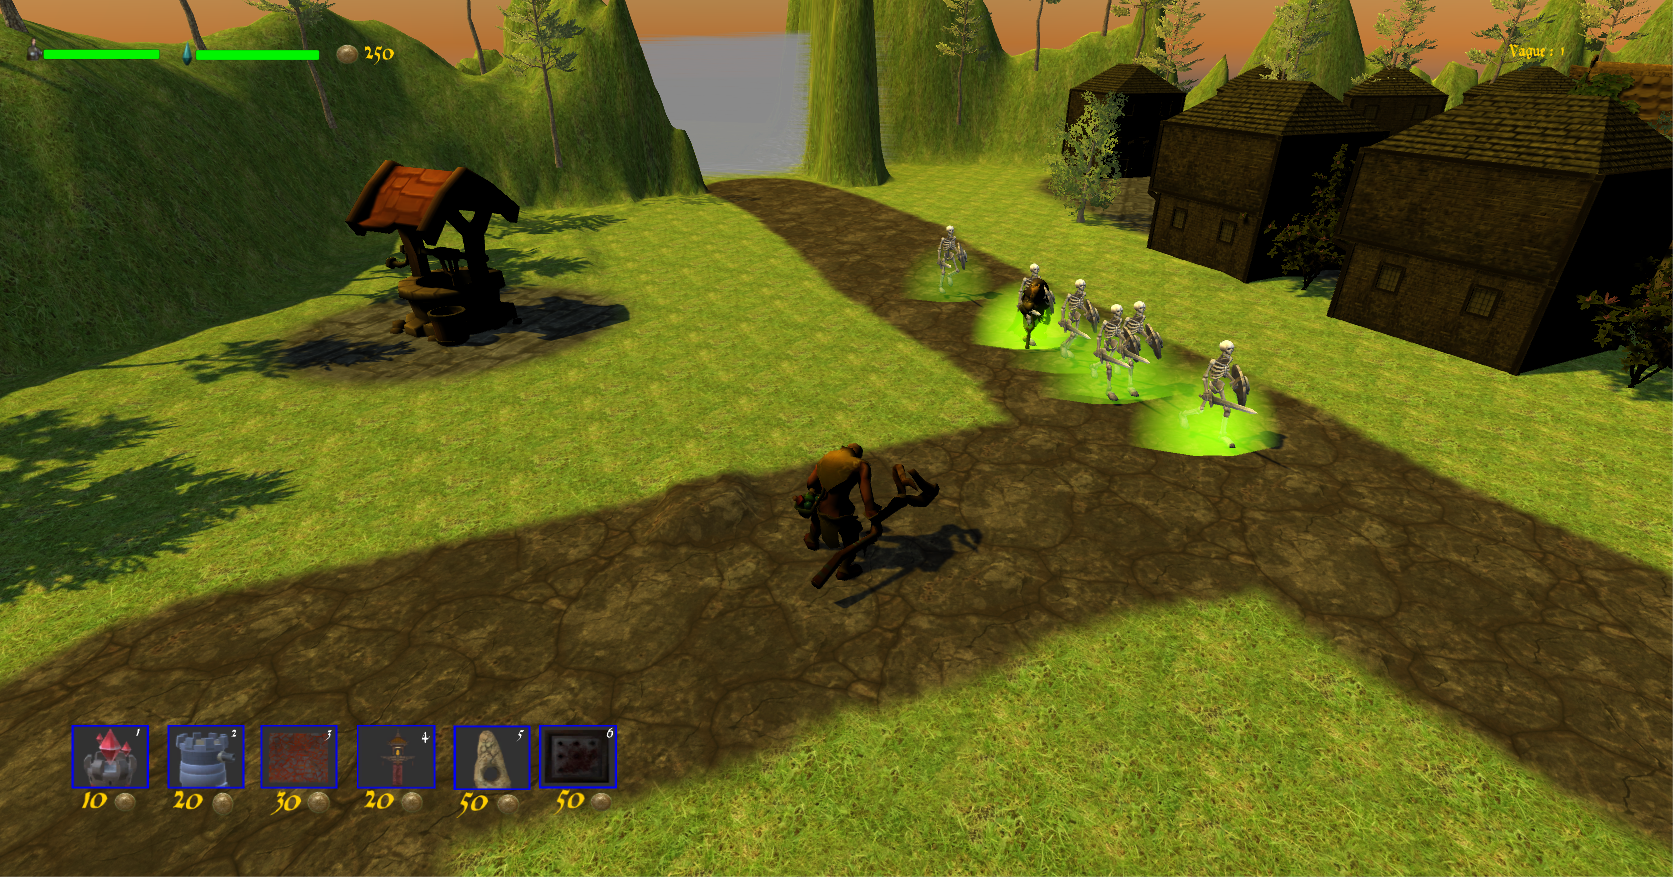
\includegraphics[scale=0.3]{Enemis.png}}
\caption*{Vague d'ennemis compos\'ee de squelettes et d'un n\'ecromancien}
\end{figure}

			\paragraph{L'arsenal défensif}
			
			L’arsenal défensif est une autre pièce majeure du gameplay de Forteresse. Il permet de repousser les ennemis et de protéger les cristaux. Il est constitué de différents types d’objets défensifs. Il existe des tours qui vont lancer des attaques, mais aussi des pièges qui vont déclencher leur effet au moment où les ennemis passent dessus. 
\par La tour arcanique est LA tour de base de Forteresse, c’est la moins ch\`ere et la plus basique de toutes les tours. Elle est apparue, en même temps que le retour de la magie dans le royaume des hommes et s’est distinguée par le fait de générer ses projectiles toute seule et donc de réduire les co\^uts liés à son utilisation. Elle possède une petite portée et de faibles dégâts, mais d’une cadence de tire relativement élevé comparé à ses sœurs, ce qui lui donne un avantage certain contre les ennemis avec peu de points de vie. Elle est donc idéale pour les débuts de partie.
\par La tour canon était la tour la plus répandue avant l’avènement de la tour arcanique. Elle fonctionne sans magie et est donc plus ch\`ere puisque nécessiteuse en projectiles. Bien qu’elle soit plus ch\`ere, elle possède de nombreux avantage comparé à sa sœur magique. La tour canon possède une portée nettement supérieure à la tour arcanique et des dégâts bien plus importants, en revanche elle possède une cadence de tire nettement ralentit par les temps de rechargement. Cela fait d’elle un atout de taille lorsqu’il faut affronter d’imposants ennemis, tels que les trolls.
\par La tour de givre est peu répandue. Elle n’est que pure magie et est difficile à ma\^itriser. Elle fait très peu de dégâts, mais ce n’est pas sa fonction première, en effet ses projectiles ralentissent les cibles qu’ils touchent. Elle possède toute fois, une vitesse d’attaque élevée et d’une portée moyenne permettant de ralentir au mieux les ennemis. Cette tours est idéale contre les monstres possédant beaucoup de points de vie, elle permet de les ralentir dans des zones de la carte o\`u sont positionnées de nombreuse tours afin de maximiser les dégâts.
\par Les tours de feu sont une invention purement humaine, ayant pour but de carboniser tout se trouvant à sa proximité. Elle crache du feu dans un cône en direction des ennemis. Elle inflige peu de dégâts, mais fait des dégâts de zone, c’est-à-dire qu’elle peut toucher plusieurs cibles en même temps. De plus tous les ennemis touchés par les flammes subissent des dégâts d’enflamment sur la durée. La tour de feu est donc très efficace pour lutter contre les grands nombres d’ennemis avec de faible points de vie, mais sera peu efficace contre les gros monstres tels que les trolls.
\par Les sols de braises sont des braises disposées au sol, ces braises infligent des dégâts conséquents, notamment sur la durée. Souvent couplé avec les tours de givre, elles sont utilisées pour réduire à néant les importantes vagues d’ennemis.
\par Les pièges d’étourdissements, à l’origine utilisé pour la chasse, puis comme pièges pour défendre les châteaux et les chambres fortes, sont désormais utilis\'e à la guerre pour tendre des embuscades aux ennemis. Ils permettent d’étourdir les ennemis pendant quelques secondes. Cependant, certains ennemis malins et résistants peuvent ne pas être affectés par les effets de ce dernier.
\par Les pierres runiques sont des objets magiques qui émettent une aura, qui améliore le rechargement des tours, leur octroyant donc une meilleure vitesse d’attaque. Toutes les tours affectées par leur effet disposent d’un halo bleu, signe de leur affectation par la magie.
\begin{figure}[!ht]
\centerline{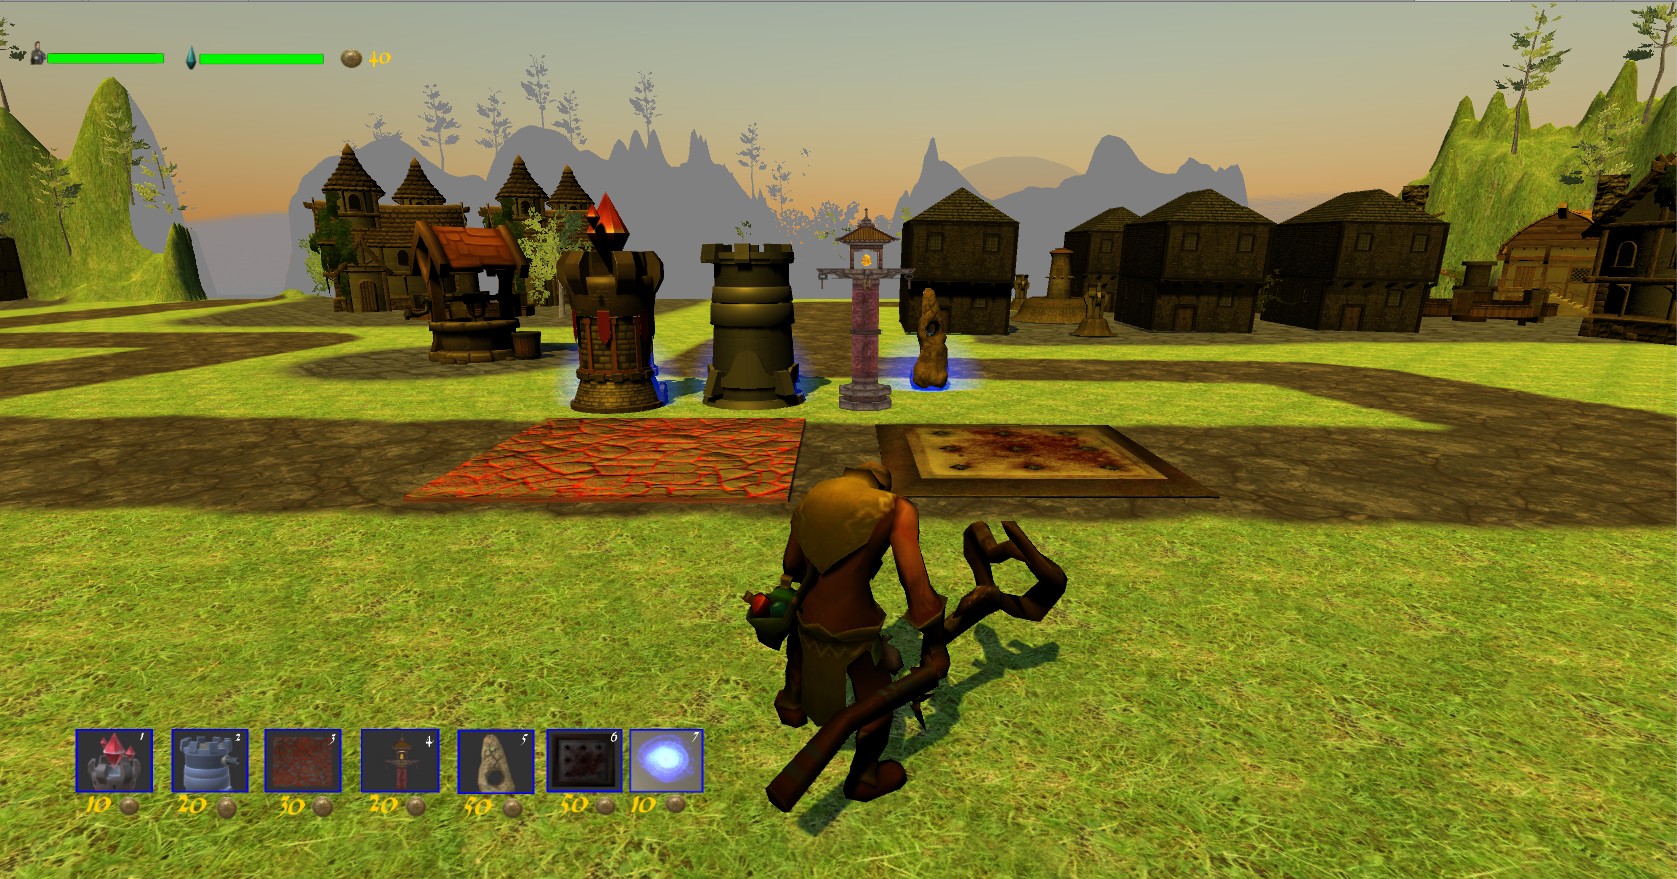
\includegraphics[scale=0.3]{Tours.png}}
\caption*{L'arsenal defensif de Forteresse}
\end{figure}
			\paragraph{Les vagues}
			
			Forteresse base tout son principe d’apparition d’ennemis sur ce que l’on appelle, des vagues. Une vague, qu’est-ce que c’est ? C’est un certain nombre d’ennemis qui vont apparaitre à certains endroits de la carte, avec une certaine cadence. Nos cartes possèdent diffèrents points d’apparitions, desquels les monstres de la vague apparaissent.
Plus on avance dans le nombre des vagues, plus des ennemis puissants comme les trolls ou les nécromanciens apparaissent, mais ce n’est pas tout ! Vous trouvez également logique que les squelettes présents dans la première vague soient moins puissants que ceux présents dans la dernière, c’est pour cela qu’à chaque vague les ennemis gagnent en résistance.
			\paragraph{Les améliorations}
			A l’origine, nous voulions créer un système d’équipement, mais cela ne correspondait pas vraiment à ce que nous voulions. Un système d’équipement aurait donné trop d’importance au personnage, or notre jeu se veut un \textit{tower defense}. Nous avons donc remanié le concept, en transformant l’équipement en amélioration temporaire. Ils sont présents pour donner un petit avantage temporaire au joueur, lui permettant possiblement de passer un vague à laquelle il aurait échoué sinon. Ces améliorations s’obtiennent en tuant des ennemis, à chaque mort d’un ennemi, vous avez un petit pourcentage de chance de voir apparaitre une amélioration. Il existe quatre améliorations différentes.
\par La premi\`ere restaure des points de vie sur la durée, il permet de rester en vie tout en prenant des risques dans les moments les plus tendus.
\par La seconde permet d’augmenter la vitesse de déplacement, très utile au vu de la taille des cartes. Il permettra d’apporter du soutient avec son personnage a plusieurs endroit diffèrent de manière plus efficace.
\par La troisième permet d’augmenter la vitesse d’attaque, cela permet à votre personnage, notamment le mage, d’infliger des dégâts considérables.
La derni\`ere augmente simplement les dégâts infligés par les personnages. Il est plus intéressant pour le guerrier qui inflige des dégâts de zone au corps à corps.

			\paragraph{Les effets visuel}
			
			Négligeable aux premiers abords mais essentiel, les effets visuels permettent au jeu de gagner en clarté. Il existe des effets sur les ennemis et sur les tours. 
Le premier effet sur les ennemis est l’effet de feu, en effet lorsqu’un ennemi est affecté par le malus de feu infligé par la tour de feu, il prend une couleur rougeâtre jusqu’à la fin du malus.
Vient ensuite dans le même esprit le changement de couleur lorsque l’ennemi est affecté par le malus de déplacement causé par la tour de givre. Il prend alors une couleur bleuté jusqu’à la fin du malus.
\par Les nécromanciens possèdent un halo de lumière verte autour d’eux pour signifier le fait qu’ils possèdent une aura. Cette lumière se retrouve sur tous les squelettes affectés par l’aura d’un nécromancien. 
\par Les effets visuels sont également importants sur les tours. A peu près dans le même esprit on retrouve une aura bleue autour des pierres runiques (elles possèdent une aura) et donc également sur toutes les tours a portée de la pierre runique. Cet effet est donc pratique pour savoir quelle sont les tours à portées de la pierre runique.
\par Les effets sont également importants sur les tours lors de la pose de celles-ci. En effet on ne peut pas poser des tours partout sur la carte, il faut donc indiquer au joueur ou il peut sinon il va vite se lasser. Les couleurs de la tour changent donc en fonction de si on peut la poser (vert) ou pas (rouge). Afin de faciliter et d’augmenter l’efficacité de la pose des pierres runiques, lors de la pose les tours à portée de la pierre prennent une couleur bleue.

			\paragraph{Les caméras}
			
			Dans tous les jeux la gestion des caméras est importante puisque c’est ce que va voir le joueur affiché sur son écran. Dans Forteresse, il existe des caméras présentes dans les menus mais nous ne parlerons pas de celles-ci dans cette partie, puisque ne faisant pas partie intégrante du gameplay. Les cameras qui nous intéresserons seront donc celles présentes lors de la partie.
\par Il y a tout d’abord la plus importante des caméras, celle du joueur. Elle va donc être un élément capital dans l’expérience que le joueur va vivre en jouant au jeu. Cette camera est capable de suivre le joueur de dos, que ce soit dans ses déplacements ou ses rotations. Notre caméra est également capable de modifier sa distance à laquelle elle est du personnage, afin de laisser au joueur régler sa propre distance en fonction de ses préférences \`a l'aide de la molette de la souris. 
\par La seconde caméra à intervenir lors d’une partie est la caméra de mort. Cette caméra est activée en cas de décès du personnage. En effet, lors de la mort du personnage celui-ci disparait. La caméra principale n’a donc plus aucun personnage à suivre. Le jeu passe donc sur une autre caméra (la caméra de mort) qui offre une vue d’ensemble de la carte en attendant la réapparition.

		\subsubsection{Le Réseau}
		Je ne me suis pas directement occupé du réseau. J’étais présent en soutien et pour apporter diverses modifications aux scripts du jeu pour leur permettre de fonctionner en réseau. En effet, le fonctionnement du jeu en réseau est très diffèrent de son fonctionnement en mode solo. Riday, a donc dû modifier de façon important l’organisation et le fonctionnement du jeu. Cela a eu pour conséquences que des scripts, qui fonctionnaient alors jusque-là très bien se sont mis à ne plus faire ce pour quoi ils ont été créé. Il a fallu refaire des versions modifiées de certains script afin qu’ils puissent fonctionner avec le réseau. C’est ici que s’est située ma tâche. J’ai donc aidé Riday en adaptant les scripts à ses besoins pour rendre le réseau fonctionnel.
		
		\subsubsection{Les Menus}
		
		A nouveau, les menus ne sont pas l’une de mes attributions principale, mais j’ai tout de même apporté ma contribution dans la réalisation de certains d’entre eux.
\par Le premier menu sur lequel j’ai travaillé avec Arnaud, est le menu pause. Je me suis occupé dans un premier temps du curseur de la souris. En effet, cela peut sembler anodin mais dans Forteresse le curseur de la souris n’est pas nécessaire lors d’une partie, il va donc gêner le joueur il a donc fallu le faire disparaitre. Ensuite certain problème de caméra et de déplacement était à régler. Le joueur pouvait déplacer son personnage et sa caméra même lorsqu’il était en mode pause. Ceci étant bien évidemment pas souhaité, le problème a donc dû être réglé. 
\par Le second menu, celui sur lequel j’ai le plus travaillé toujours en collaboration avec Arnaud, est le menu de sélection des personnages. Ce menu permet comme son nom l’indique de sélectionner le personnage que l’on souhaite jouer (le mage ou le guerrier). Il a donc fallu de dans un premier temps créer l’environnement graphique du menu, ce fut la partie simple du menu. Il a ensuite fallu faire en sorte de pouvoir sélectionner le personnage souhaité. Et enfin la partie la plus dure a été de gérer l’apparition du curseur en fonction du mode pause, puisque lors de la sélection des personnages, le jeu est sur pause mais le curseur est visible. Cela a causé de nombreux problème avec le menu pause, notamment des conflits entre le mode pause et la visibilité du curseur.

			\subsubsection{Le multijoueur}
			En ce qui concerne le multijoueur notre jeu ne possède pas de changement de mode particulier. Le déroulement d’une partie est le même, simplement les joueurs sont plusieurs aux lieux d’être seul dans la partie. Il y a donc un avantage certain à jouer à plusieurs.
				
			
\section{Bilan personnel}
	\subsection{\textsc{Chatelus} Florian}
	Après 6 mois de travail sur ce projet, voici le bilan que j’ai pu en tirer. Pour moi il y a eu trois points sur lesquels j’ai dû travailler pendant la durée de ce projet, le premier est l’aspect autodidacte du projet, vient ensuite la contrainte des dates limites et pour finir la gestion du travail de groupe.
		\medbreak
\par Je dois bien avouer qu’au départ, en tout début d’année lorsque les spés sont venues nous parler de leurs jeux, un tel projet m’avait semblé facile en dépit de tous leurs avertissements. Je me rappelle encore les entendre dire que leur jeu marchait mais que ce n’était qu’en apparence, qu’il y avait des bugs mais qu’ils s’étaient débrouillé pour les cacher et que si nous pensions faire un jeu sans bug, il fallait arrêter de rêver tout de suite car ça n’allait pas arriver. Bien évidement en tant que sup tout juste sortie de terminal je m’imaginais déjà avoir un jeu parfait sans bug et qui serait magnifique. Bien évidemment ce n’est absolument pas comme cela que ça s’est passé, je n’avais pas réalisé que nous allions être totalement sans aide du début à la fin. A l’arrivé au deuxième semestre tout est allé très vite et malgré les conférences faites pour nous aider, le début de notre projet ne se fit pas sans mal. En effet, il a fallu tout d’abord apprendre à utiliser git afin de pouvoir échanger notre travail. La particularité de git est qu’il s’utilise en console, alors nous qui n’avions jamais utilisé une console auparavant, nous avons eu beaucoup de mal a seulement maitriser les bases de git. Et ce n’est qu’après des heures d’essai et de tutoriels que nous avons finalement réussi à utiliser des fonctions de base de git, je ne parle bien évidemment pas de la résolution de problème que nous avons pu rencontrer. Ce fut ma première leçon d’humilité, nous n’avions même pas commencé quoi que ce soit et nous étions déjà perdus. Mais l’utilisation de git n’était qu’une mise en bouche, les vrai difficultés sont apparues avec l’arrivé de Unity. Là, o\`u pour git il n’y avait que quelques commandes à apprendre, là, c’était tout un moteur graphique, alors bien évidemment, je ne le maitrise toujours pas à 100\%  mais je pense tout de même avoir une certaine expérience sur le moteur, qui me permet de ne plus me considérer comme un novice bien que je n’en sois pas loin. Je pense que cela m’a permis d’améliorer la façon dont je fais mes recherches et avec laquelle j’appréhende les outils qui me sont inconnus.
	\medbreak
\par Bien évidemment l’apprentissage de tous ces nouveaux outils sont très chronophages bien que certains comme Unity sont réputés facile à prendre en main. La gestion des dates butoirs furent également un défi. Les délais étaient très courts notamment au début, l’écriture du cahier des charges a dû se faire très rapidement, de plus, il fallait se mettre d’accord avec tout le groupe. Je pense que je suis quelqu’un de plutôt organis\'e et sérieux, je n’ai donc pas eu trop de mal à tenir mes délais. Mais le projet demande tout de même une certaine charge de travail, j’ai donc été forcé de travailler de façon régulière et efficace, chose que je ne faisais pas systématiquement auparavant. Avoir un projet en parallèle des cours a donc été intéressant, puisque tous deux étaient parfaitement indépendants. Il a donc fallu adopter le bon équilibre entre travail sur le projet et travail des cours. Cet équilibre n’a pas forcement été simple à trouver étant donné que j’avais une large préférence pour la réalisation du projet. Il faut bien l’avouer, réaliser un jeu vidéo est plus intéressant qu’un espace vectoriel. La préparation des soutenances aussi furent compliquées en termes de délais, cela n’a rien à voir avec un exposé classique puisque dans le cas d’une soutenance, c’est nous qui créons la matière que nous allons utiliser. Cela a donc été très motivant pour moi, plus j’en faisais, plus simple serait pour moi la soutenance puisqu’il est plus facile de parler de choses intéressantes que de remplir les quelques minutes de prise de parole avec du vide. Mais c’est un travail de groupe, donc toute la difficulté réside dans le fait que si un membre du groupe flanche, tout le groupe flanche.
	\medbreak
\par Malheureusement pour nous, un membre du groupe, Yassine, a choisi de quitter l’EPTA quelques semaines après le début du projet, nous nous sommes donc rapidement retrouvés à trois. Ce fut un coup dur. Malgré son départ prématuré il a été présent lors de la réalisation du cahier des charges, j’ai donc pour la première fois durant le projet d\^u composer avec les membres de mon groupe, notamment pour le choix du jeu que nous allions réaliser. Je n’avais pas trop eu ce problème en terminal lors de mon projet en ISN puisque j’avais une attitude assez passive vis-à-vis du projet. Au finale, j’ai quasiment imposé ma vision du jeu à notre groupe, après coup je ne regrette pas d’avoir fait cela car je pense avoir été le meneur du groupe. Avec un départ du groupe et Arnaud et Riday jouant peu voir jamais à des jeux vidéo j’étais donc le plus apte à savoir dans quelle direction nous devions aller pour créer un jeu vidéo. Cette expérience de meneur fut très enrichissante étant donné qu’en générale je suis plutôt la personne que l’on doit porter tout le long d’un projet. J’ai aimé pousser et aider mes camarades tout le long du projet. Je pense que ceci est un gros point positif de ce projet, même si mes encouragements peuvent parfois tomber dans le harcèlement, c’est donc quelque chose qu’il me reste encore à travailler et que j’espère mieux maitriser à l’avenir.
	\medbreak
\par Ce projet m’a donc permis de travailler sur plusieurs compétences. La première est celle que je pense être la plus importante surtout pour un étudiant est l’auto-apprentissage, on a fait comme on pouvait avec ce qu’on savait. Ensuite vient la gestion de son temps, chose qui deviendra capital dans les années à venir. Et pour conclure, le travail de groupe est indispensable dans bien des domaines et ne présente quasiment que des points positifs.

	\subsection{\textsc{Henric} Arnaud}
	
	Le projet de cette année d’Info-Sup à Epita a été une expérience très enrichissante sur différents plans.
\medbreak
\par D’abord, il m’a appris à travailler en groupe. Ce n’est certes pas la première fois que je réalise un travail en groupe puisque nous avons eu le TPE à faire pour le bac en première mais c’est le premier travail en groupe qui demandait une quantité de travail aussi importante. De plus, nous devions travailler régulièrement étant donné qu’on avait trois soutenances durant le semestre, ce qui fait peu de temps entre chaque présentation. Je trouve d’ailleurs cette organisation intéressante car elle nous empêche de tout programmer la dernière semaine et donc d’avoir un jeu fonctionnel avec un certain temps pour régler les problèmes. Ensuite, j’ai apprécié travailler en groupe notamment parce qu’on avait une bonne équipe et on tous su se mettre au travail et bien répartir les tâches. De plus, nous étions soudés et nous nous entraidions même pour des parties qui n’étaient pas les n\^otres. On voulait, chacun d’entre nous, réussir à réaliser un bon projet et cela ne pouvait être que bénéfique pour le bon déroulement de la réalisation de notre jeu. En tant que chef de groupe, je suis très satisfait de chacun et je pense que l’organisation et la répartition des tâches étaient optimale.
\medbreak
\par Dans un second temps, le projet est un bon moyen de se rendre compte réellement de ce que l’on peut réaliser en informatique. On peut se mettre à la place des développeurs et comprendre une partie de leur métier. C’est un excellent “test” en première année pour savoir si on suit la bonne voie et je me suis bien rendu compte qu’EPITA était vraiment l’école où je souhaitais aller. Un jeu vidéo est un thème assez libre, et la réalisation de celui-ci demande des connaissances assez diverses. Savoir faire fonctionner une IA, créer un menu et développer un système de réseau sans avoir beaucoup de bases en informatique en cette première année demandait beaucoup de travail. Néanmoins, c’est un point positif car un ingénieur doit savoir se débrouiller et chercher les informations sur internet ou d’autres supports pour faire avancer son projet.
\medbreak
\par Plongés au coeur du métier d’ingénieur informatique, nous avions également des soutenances. On peut, encore une fois, se mettre à la place d’un développeur qui, après avoir réaliser son projet, doit vendre son produit et en faire la publicité. Je pense que les soutenances se rapprochaient vraiment de cette partie commerciale, puisqu’on essayait de montrer les points positifs de notre jeu et de donner envie au publique de le télécharger. Les soutenances nous ont également entraîné à nous exprimer à l’oral. Plus tard, nous auront sûrement des présentations à faire et il est très important de se préparer dès le but du cycle à EPITA. 
\medbreak
\par Enfin, on peut s’estimer chanceux de pouvoir utiliser des outils fabuleux comme Unity qui n’existaient pas quelques années auparavant. C’est un bonheur de pouvoir manipuler des objets en 3D et de créer des montres et des terrains de jeu aussi jolis et avec efficacité. Les outils comme Git nous ont aussi été très utiles afin de partager rapidement nos modifications sur le projet pour que tout le monde puisse travailler chez soi.
\medbreak
\par En conclusion, ce projet de première année à EPITA était vraiment plaisant à réaliser. Nous avons eu accès à des outils complexes mais offrant beaucoup de liberté et permettant d’obtenir un beau rendu. Ce projet nous est bénéfique pour l’avenir, il nous a rapproché du métier d’ingénieur et nous a permis d’apprendre à travailler en groupe. Je suis donc ravi d’avoir créé Forteresse.

\subsection{\textsc{Sarkar} Riday}


\par La proposition de réaliser un jeu vidéo en tant que projet de fin d’année plaît à un bon nombre d’élèves de première année. La plupart d’entre eux ont surement passé beaucoup du temps avec les jeux-vidéos mais ce n’était pas mon cas. Etant donné que je passe très peu de temps avec les jeux-vidéos, je savais que ce projet allait me permettre d’apprendre beaucoup de choses sur les jeux-vidéos. Ce projet m’a enthousiasmé dès le début.
\medbreak
\par Ce projet m’a apporté beaucoup de choses dans beaucoup de domaines notamment le travail en groupe. En effet, j’avais déjà réalisé un travail en groupe dans le cadre du TPE lorsque j’étais en première mais ce projet est d’une ampleur totalement différente et nécessite une méthode du travail totalement différente avec une autre approche du travail en groupe.
\medbreak
\par Avec ce projet, j’ai appris que travailler en groupe n’est pas aussi simple que je le pensais avant de commencer ce projet. Lorsqu’on travaille en groupe, il faut que tous les membres du groupe proposent des idées pour l’avancement du projet mais il faut accepter le fait que les idées que l’on propose ne plaisent pas toujours aux autres. On peut avoir des opinions qui divergent au sein d’un même groupe. Donc lorsqu’on réalise une tâche, elle peut ne pas plaire aux autres membres du groupe.  On peut être amené à recommencer ce qu’on a fait. C’était particulièrement mon cas puisque je me suis occupé de la partie graphisme qui est une partie purement visuelle.  Avant de mettre mon travail dans le projet, je le montrais souvent à Florian qui me donnait son avis sur la qualité de mon travail. Il était très honnête et je le remercie puisqu’à chaque fois je recommençais un travail, la qualité de mon travail était meilleure. A travers la réalisation de ce projet, j’ai appris à accepter que mon travail peut parfois ne pas plaire aux autres et qu’il ne faut pas hésiter à recommencer si nécessaire.
\medbreak
\par Ce projet m’a permis aussi de contrôler mon stress.  En effet, au début du projet, je passais beaucoup du temps sur certaine tâche sans succès et je me stressais beaucoup et j’avais un sentiment d’échec. Mais au cours du projet, j’ai appris à gérer mon stress. J’ai appris que tant qu’on n’y arrive pas, il faut recommencer et on finit par y arriver. Dans un travail en équipe, il faut respecter le délai accordé pour que les autres membres du groupe puissent avancer et ne restent pas bloqués par notre travail qui était à faire. C’est très stressant lorsqu’on pense au délai qui nous a été accordé parce qu’on a peur de ne pas finir dans les temps. Dans la vie professionnelle, il faut respecter le délai qui nous a été accordé et ce projet était en quelque sorte un très bon entraînement.
\par En outre du travail en groupe, ce projet m’a permis non seulement d’appliquer les notions vues en cours dans un cas concret mais aussi d’apprendre des nouvelles choses qu’on a pas vues en cours. Avec ce projet, j’ai aussi appris à chercher des choses dont j’avais besoin pour avancer le projet. Ce projet m’a donné un avant-go\^ut au métier d’ingénieur. En effet, puisque nous ne pouvons pas tout savoir, nous, en tant qu’ingénieur, devons apprendre de nouvelles choses au cours de notre vie professionnelle. Nous devons donc savoir faire des recherches. En effet, dans un premier temps, il faut comprendre les ressources que l'on a récoltées avec nos recherches puis les réadapter avant de les appliquer dans le projet. J’ai appris donc ces diverses méthodes du travail à travers ce projet.
\medbreak
\par Enfin ce projet m’a aussi permis d’avoir de bonnes relation avec mes camarades. En effet, pour certaine partie comme la 2D et la 3D, j’étais autonome mais j’ai dû demander à mes camarades des renseignements sur la partie réseau.  Cela m’a permis d’avoir de bonnes relations avec des personnes qui ne sont pas dans mon groupe en plus de mes deux camarades du groupe. Le fait que tous les membres de notre groupe soient dans la même classe a permis de bien avancer le projet puisqu’on se voyait tous les jours. Ce projet m'a apport\'e beaucoup de choses et m'a pr\'epar\'e pour les projet a venir. 


\section{Conclusion}

Le projet \'etant enfin fini, il est maintenant disponible en t\'el\'echargement. Le groupe FARY vous invite donc \'a l'essayer d\`es maintenant si vous avez le courage. Enfilez vos armures, pr\'eparez vos armes et canalisez votre magie. Serez vous capable de prot\'eger le royaume en combattant les forces du mal que seul vous pouvez vaincre ?

\begin{figure}[!ht]
\centerline{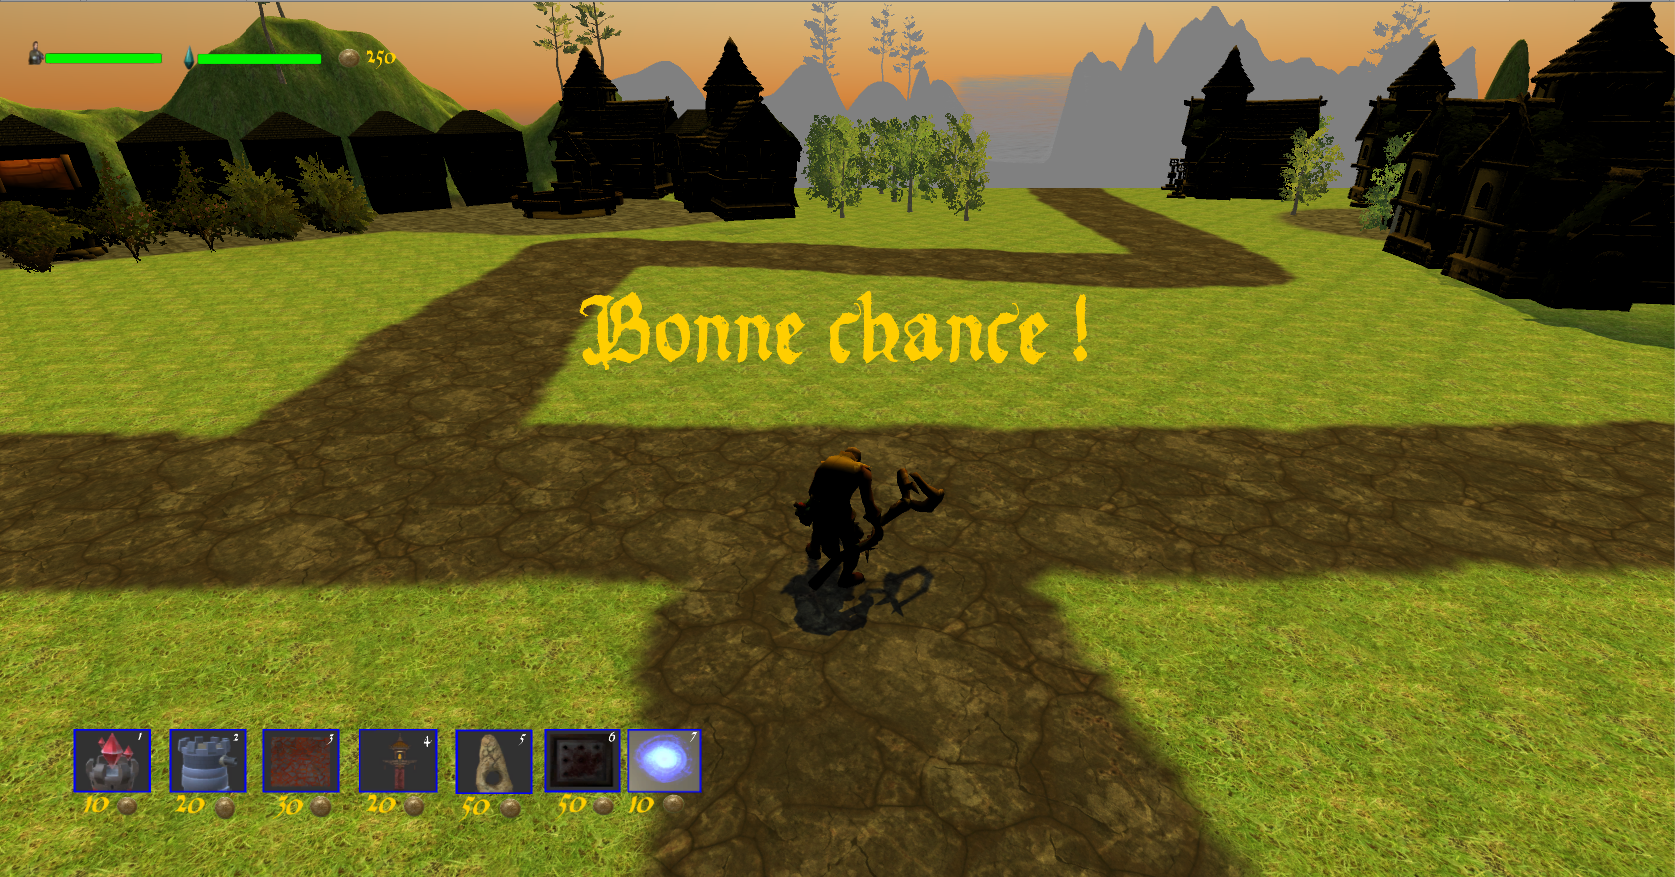
\includegraphics[scale=0.3]{BonneChance.png}}
\caption*{Bonne Chance !}
\end{figure}

\section{Annexe}
\large \textbf{Squelette}\\
\centerline{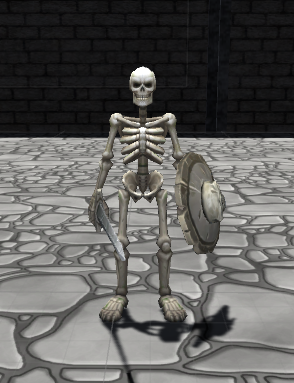
\includegraphics[scale=0.8]{Skeleton.png}}
\large \textbf{Gobelin}\\
\smallbreak
\centerline{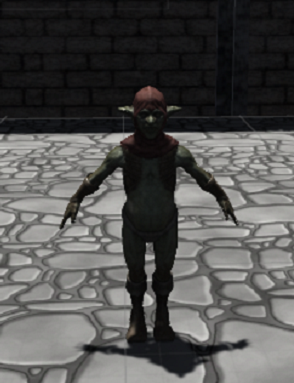
\includegraphics[scale=0.8]{Goblin.png}}
\bigbreak
\large \textbf{Troll}\\
\smallbreak
\centerline{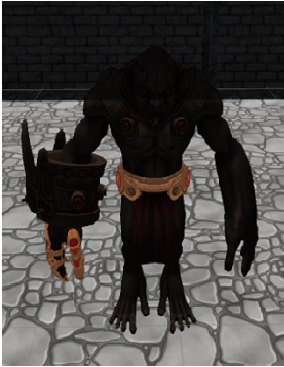
\includegraphics[scale=0.8]{Troll.png}}
\bigbreak
\large \textbf{L'archer gobelin}\\
\smallbreak
\centerline{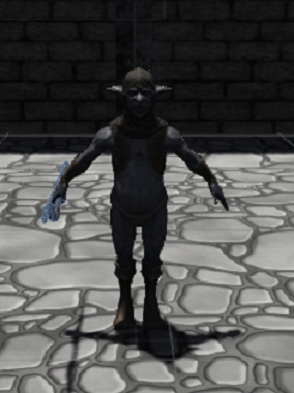
\includegraphics[scale=0.8]{Ranger.png}}
\bigbreak
\large \textbf{D\'emon des enfers}\\
\smallbreak
\centerline{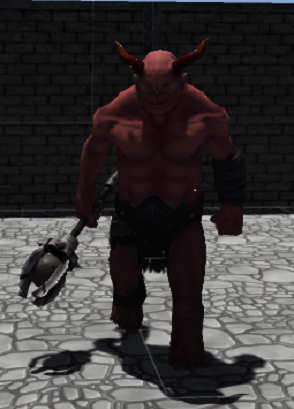
\includegraphics[scale=0.8]{HellKeeper.png}}
\bigbreak
\large \textbf{Necormancien}\\
\smallbreak
\centerline{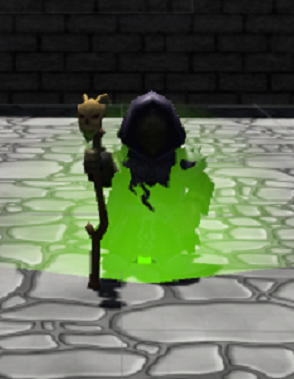
\includegraphics[scale=0.8]{Necromancer.png}}
\bigbreak
\large \textbf{Gardien}\\
\smallbreak
\centerline{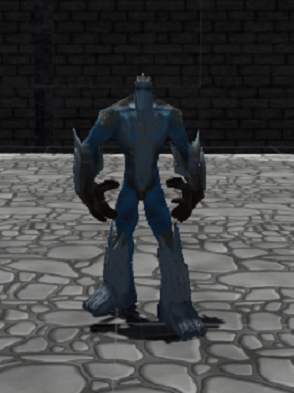
\includegraphics[scale=0.8]{Overseer.png}}
\bigbreak

\large \textbf{Tour Arcanique}
\smallbreak
\centerline{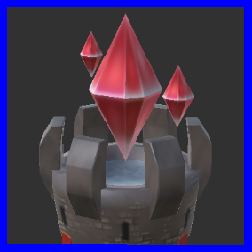
\includegraphics{Mage.png}}
\bigbreak
\newpage
\large \textbf{Tour Canon}
\smallbreak
\centerline{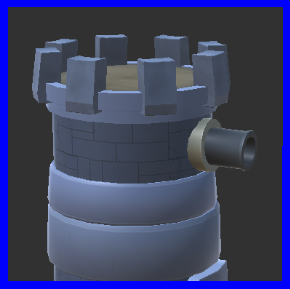
\includegraphics{Canon.png}}
\bigbreak

\large \textbf{Tour de feu}
\smallbreak
\centerline{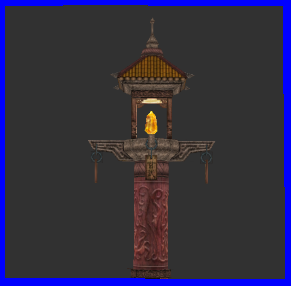
\includegraphics{FirTower.png}}
\bigbreak
\newpage

\large \textbf{Tour de givre}
\smallbreak
\centerline{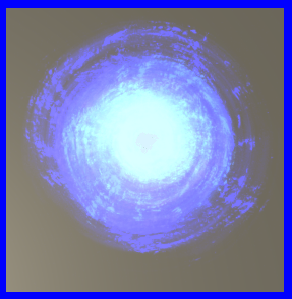
\includegraphics{IconeFrozenTower.png}}
\bigbreak

\large \textbf{Sol de braises}
\smallbreak
\centerline{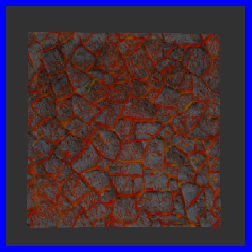
\includegraphics[scale=1.2]{LavaBrik.png}}
\bigbreak
\newpage

\large \textbf{Pi\`ege \'etourdissant}
\smallbreak
\centerline{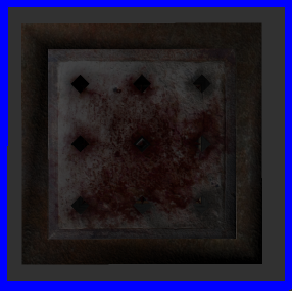
\includegraphics{fbx.png}}
\bigbreak

\newpage
\begin{spacing}{1.0}
	\tableofcontents
\end{spacing}

\end{document}
